\documentclass[twoside]{book}

% Packages required by doxygen
\usepackage{fixltx2e}
\usepackage{calc}
\usepackage{doxygen}
\usepackage[export]{adjustbox} % also loads graphicx
\usepackage{graphicx}
\usepackage[utf8]{inputenc}
\usepackage{makeidx}
\usepackage{multicol}
\usepackage{multirow}
\PassOptionsToPackage{warn}{textcomp}
\usepackage{textcomp}
\usepackage[nointegrals]{wasysym}
\usepackage[table]{xcolor}

% Font selection
\usepackage[T1]{fontenc}
\usepackage[scaled=.90]{helvet}
\usepackage{courier}
\usepackage{amssymb}
\usepackage{sectsty}
\renewcommand{\familydefault}{\sfdefault}
\allsectionsfont{%
  \fontseries{bc}\selectfont%
  \color{darkgray}%
}
\renewcommand{\DoxyLabelFont}{%
  \fontseries{bc}\selectfont%
  \color{darkgray}%
}
\newcommand{\+}{\discretionary{\mbox{\scriptsize$\hookleftarrow$}}{}{}}

% Page & text layout
\usepackage{geometry}
\geometry{%
  a4paper,%
  top=2.5cm,%
  bottom=2.5cm,%
  left=2.5cm,%
  right=2.5cm%
}
\tolerance=750
\hfuzz=15pt
\hbadness=750
\setlength{\emergencystretch}{15pt}
\setlength{\parindent}{0cm}
\setlength{\parskip}{3ex plus 2ex minus 2ex}
\makeatletter
\renewcommand{\paragraph}{%
  \@startsection{paragraph}{4}{0ex}{-1.0ex}{1.0ex}{%
    \normalfont\normalsize\bfseries\SS@parafont%
  }%
}
\renewcommand{\subparagraph}{%
  \@startsection{subparagraph}{5}{0ex}{-1.0ex}{1.0ex}{%
    \normalfont\normalsize\bfseries\SS@subparafont%
  }%
}
\makeatother

% Headers & footers
\usepackage{fancyhdr}
\pagestyle{fancyplain}
\fancyhead[LE]{\fancyplain{}{\bfseries\thepage}}
\fancyhead[CE]{\fancyplain{}{}}
\fancyhead[RE]{\fancyplain{}{\bfseries\leftmark}}
\fancyhead[LO]{\fancyplain{}{\bfseries\rightmark}}
\fancyhead[CO]{\fancyplain{}{}}
\fancyhead[RO]{\fancyplain{}{\bfseries\thepage}}
\fancyfoot[LE]{\fancyplain{}{}}
\fancyfoot[CE]{\fancyplain{}{}}
\fancyfoot[RE]{\fancyplain{}{\bfseries\scriptsize Generated by Doxygen }}
\fancyfoot[LO]{\fancyplain{}{\bfseries\scriptsize Generated by Doxygen }}
\fancyfoot[CO]{\fancyplain{}{}}
\fancyfoot[RO]{\fancyplain{}{}}
\renewcommand{\footrulewidth}{0.4pt}
\renewcommand{\chaptermark}[1]{%
  \markboth{#1}{}%
}
\renewcommand{\sectionmark}[1]{%
  \markright{\thesection\ #1}%
}

% Indices & bibliography
\usepackage{natbib}
\usepackage[titles]{tocloft}
\setcounter{tocdepth}{3}
\setcounter{secnumdepth}{5}
\makeindex

% Hyperlinks (required, but should be loaded last)
\usepackage{ifpdf}
\ifpdf
  \usepackage[pdftex,pagebackref=true]{hyperref}
\else
  \usepackage[ps2pdf,pagebackref=true]{hyperref}
\fi
\hypersetup{%
  colorlinks=true,%
  linkcolor=blue,%
  citecolor=blue,%
  unicode%
}

% Custom commands
\newcommand{\clearemptydoublepage}{%
  \newpage{\pagestyle{empty}\cleardoublepage}%
}

\usepackage{caption}
\captionsetup{labelsep=space,justification=centering,font={bf},singlelinecheck=off,skip=4pt,position=top}

%===== C O N T E N T S =====

\begin{document}

% Titlepage & ToC
\hypersetup{pageanchor=false,
             bookmarksnumbered=true,
             pdfencoding=unicode
            }
\pagenumbering{alph}
\begin{titlepage}
\vspace*{7cm}
\begin{center}%
{\Large Gliese }\\
\vspace*{1cm}
{\large Generated by Doxygen 1.8.13}\\
\end{center}
\end{titlepage}
\clearemptydoublepage
\pagenumbering{roman}
\tableofcontents
\clearemptydoublepage
\pagenumbering{arabic}
\hypersetup{pageanchor=true}

%--- Begin generated contents ---
\chapter{Namespace Index}
\section{Packages}
Here are the packages with brief descriptions (if available)\+:\begin{DoxyCompactList}
\item\contentsline{section}{\hyperlink{namespace_t_d_j___gliese}{T\+D\+J\+\_\+\+Gliese} }{\pageref{namespace_t_d_j___gliese}}{}
\item\contentsline{section}{\hyperlink{namespace_t_d_j___gliese_1_1_content}{T\+D\+J\+\_\+\+Gliese.\+Content} }{\pageref{namespace_t_d_j___gliese_1_1_content}}{}
\end{DoxyCompactList}

\chapter{Hierarchical Index}
\section{Class Hierarchy}
This inheritance list is sorted roughly, but not completely, alphabetically\+:\begin{DoxyCompactList}
\item \contentsline{section}{T\+D\+J\+\_\+\+Gliese.\+Content.\+Boom}{\pageref{class_t_d_j___gliese_1_1_content_1_1_boom}}{}
\item \contentsline{section}{T\+D\+J\+\_\+\+Gliese.\+Button}{\pageref{class_t_d_j___gliese_1_1_button}}{}
\item \contentsline{section}{T\+D\+J\+\_\+\+Gliese.\+Enemy\+Ship}{\pageref{class_t_d_j___gliese_1_1_enemy_ship}}{}
\item Game\begin{DoxyCompactList}
\item \contentsline{section}{T\+D\+J\+\_\+\+Gliese.\+Game1}{\pageref{class_t_d_j___gliese_1_1_game1}}{}
\end{DoxyCompactList}
\item \contentsline{section}{T\+D\+J\+\_\+\+Gliese.\+L\+VL}{\pageref{class_t_d_j___gliese_1_1_l_v_l}}{}
\item \contentsline{section}{T\+D\+J\+\_\+\+Gliese.\+Pause\+Menu}{\pageref{class_t_d_j___gliese_1_1_pause_menu}}{}
\item \contentsline{section}{T\+D\+J\+\_\+\+Gliese.\+Power\+Up}{\pageref{class_t_d_j___gliese_1_1_power_up}}{}
\item \contentsline{section}{T\+D\+J\+\_\+\+Gliese.\+Projectile}{\pageref{class_t_d_j___gliese_1_1_projectile}}{}
\item \contentsline{section}{T\+D\+J\+\_\+\+Gliese.\+Ship}{\pageref{class_t_d_j___gliese_1_1_ship}}{}
\item \contentsline{section}{T\+D\+J\+\_\+\+Gliese.\+Space\+\_\+\+Back\+Ground}{\pageref{class_t_d_j___gliese_1_1_space___back_ground}}{}
\end{DoxyCompactList}

\chapter{Class Index}
\section{Class List}
Here are the classes, structs, unions and interfaces with brief descriptions\+:\begin{DoxyCompactList}
\item\contentsline{section}{\hyperlink{class_t_d_j___gliese_1_1_content_1_1_boom}{T\+D\+J\+\_\+\+Gliese.\+Content.\+Boom} }{\pageref{class_t_d_j___gliese_1_1_content_1_1_boom}}{}
\item\contentsline{section}{\hyperlink{class_t_d_j___gliese_1_1_button}{T\+D\+J\+\_\+\+Gliese.\+Button} }{\pageref{class_t_d_j___gliese_1_1_button}}{}
\item\contentsline{section}{\hyperlink{class_t_d_j___gliese_1_1_enemy_ship}{T\+D\+J\+\_\+\+Gliese.\+Enemy\+Ship} }{\pageref{class_t_d_j___gliese_1_1_enemy_ship}}{}
\item\contentsline{section}{\hyperlink{class_t_d_j___gliese_1_1_game1}{T\+D\+J\+\_\+\+Gliese.\+Game1} }{\pageref{class_t_d_j___gliese_1_1_game1}}{}
\item\contentsline{section}{\hyperlink{class_t_d_j___gliese_1_1_l_v_l}{T\+D\+J\+\_\+\+Gliese.\+L\+VL} }{\pageref{class_t_d_j___gliese_1_1_l_v_l}}{}
\item\contentsline{section}{\hyperlink{class_t_d_j___gliese_1_1_pause_menu}{T\+D\+J\+\_\+\+Gliese.\+Pause\+Menu} }{\pageref{class_t_d_j___gliese_1_1_pause_menu}}{}
\item\contentsline{section}{\hyperlink{class_t_d_j___gliese_1_1_power_up}{T\+D\+J\+\_\+\+Gliese.\+Power\+Up} }{\pageref{class_t_d_j___gliese_1_1_power_up}}{}
\item\contentsline{section}{\hyperlink{class_t_d_j___gliese_1_1_projectile}{T\+D\+J\+\_\+\+Gliese.\+Projectile} }{\pageref{class_t_d_j___gliese_1_1_projectile}}{}
\item\contentsline{section}{\hyperlink{class_t_d_j___gliese_1_1_ship}{T\+D\+J\+\_\+\+Gliese.\+Ship} }{\pageref{class_t_d_j___gliese_1_1_ship}}{}
\item\contentsline{section}{\hyperlink{class_t_d_j___gliese_1_1_space___back_ground}{T\+D\+J\+\_\+\+Gliese.\+Space\+\_\+\+Back\+Ground} }{\pageref{class_t_d_j___gliese_1_1_space___back_ground}}{}
\end{DoxyCompactList}

\chapter{File Index}
\section{File List}
Here is a list of all files with brief descriptions\+:\begin{DoxyCompactList}
\item\contentsline{section}{T\+D\+J-\/\+Gliese/\hyperlink{_boom_8cs}{Boom.\+cs} }{\pageref{_boom_8cs}}{}
\item\contentsline{section}{T\+D\+J-\/\+Gliese/\hyperlink{_button_8cs}{Button.\+cs} }{\pageref{_button_8cs}}{}
\item\contentsline{section}{T\+D\+J-\/\+Gliese/\hyperlink{_enemy_ship_8cs}{Enemy\+Ship.\+cs} }{\pageref{_enemy_ship_8cs}}{}
\item\contentsline{section}{T\+D\+J-\/\+Gliese/\hyperlink{_game1_8cs}{Game1.\+cs} }{\pageref{_game1_8cs}}{}
\item\contentsline{section}{T\+D\+J-\/\+Gliese/\hyperlink{_l_v_l_8cs}{L\+V\+L.\+cs} }{\pageref{_l_v_l_8cs}}{}
\item\contentsline{section}{T\+D\+J-\/\+Gliese/\hyperlink{_pause_menu_8cs}{Pause\+Menu.\+cs} }{\pageref{_pause_menu_8cs}}{}
\item\contentsline{section}{T\+D\+J-\/\+Gliese/\hyperlink{_power_up_8cs}{Power\+Up.\+cs} }{\pageref{_power_up_8cs}}{}
\item\contentsline{section}{T\+D\+J-\/\+Gliese/\hyperlink{_program_8cs}{Program.\+cs} }{\pageref{_program_8cs}}{}
\item\contentsline{section}{T\+D\+J-\/\+Gliese/\hyperlink{_projectile_8cs}{Projectile.\+cs} }{\pageref{_projectile_8cs}}{}
\item\contentsline{section}{T\+D\+J-\/\+Gliese/\hyperlink{_ship_8cs}{Ship.\+cs} }{\pageref{_ship_8cs}}{}
\item\contentsline{section}{T\+D\+J-\/\+Gliese/\hyperlink{_space___back_ground_8cs}{Space\+\_\+\+Back\+Ground.\+cs} }{\pageref{_space___back_ground_8cs}}{}
\item\contentsline{section}{T\+D\+J-\/\+Gliese/\+Properties/\hyperlink{_assembly_info_8cs}{Assembly\+Info.\+cs} }{\pageref{_assembly_info_8cs}}{}
\end{DoxyCompactList}

\chapter{Namespace Documentation}
\hypertarget{namespace_t_d_j___gliese}{}\section{T\+D\+J\+\_\+\+Gliese Namespace Reference}
\label{namespace_t_d_j___gliese}\index{T\+D\+J\+\_\+\+Gliese@{T\+D\+J\+\_\+\+Gliese}}
\subsection*{Namespaces}
\begin{DoxyCompactItemize}
\item 
namespace \hyperlink{namespace_t_d_j___gliese_1_1_content}{Content}
\end{DoxyCompactItemize}
\subsection*{Classes}
\begin{DoxyCompactItemize}
\item 
class \hyperlink{class_t_d_j___gliese_1_1_button}{Button}
\item 
class \hyperlink{class_t_d_j___gliese_1_1_enemy_ship}{Enemy\+Ship}
\item 
class \hyperlink{class_t_d_j___gliese_1_1_game1}{Game1}
\item 
class \hyperlink{class_t_d_j___gliese_1_1_l_v_l}{L\+VL}
\item 
class \hyperlink{class_t_d_j___gliese_1_1_pause_menu}{Pause\+Menu}
\item 
class \hyperlink{class_t_d_j___gliese_1_1_power_up}{Power\+Up}
\item 
class \hyperlink{class_t_d_j___gliese_1_1_projectile}{Projectile}
\item 
class \hyperlink{class_t_d_j___gliese_1_1_ship}{Ship}
\item 
class \hyperlink{class_t_d_j___gliese_1_1_space___back_ground}{Space\+\_\+\+Back\+Ground}
\end{DoxyCompactItemize}

\hypertarget{namespace_t_d_j___gliese_1_1_content}{}\section{T\+D\+J\+\_\+\+Gliese.\+Content Namespace Reference}
\label{namespace_t_d_j___gliese_1_1_content}\index{T\+D\+J\+\_\+\+Gliese.\+Content@{T\+D\+J\+\_\+\+Gliese.\+Content}}
\subsection*{Classes}
\begin{DoxyCompactItemize}
\item 
class \hyperlink{class_t_d_j___gliese_1_1_content_1_1_boom}{Boom}
\end{DoxyCompactItemize}

\chapter{Class Documentation}
\hypertarget{class_t_d_j___gliese_1_1_content_1_1_boom}{}\section{T\+D\+J\+\_\+\+Gliese.\+Content.\+Boom Class Reference}
\label{class_t_d_j___gliese_1_1_content_1_1_boom}\index{T\+D\+J\+\_\+\+Gliese.\+Content.\+Boom@{T\+D\+J\+\_\+\+Gliese.\+Content.\+Boom}}
\subsection*{Public Member Functions}
\begin{DoxyCompactItemize}
\item 
\hyperlink{class_t_d_j___gliese_1_1_content_1_1_boom_aa0a4164c674f545a310cd04810f9921c}{Boom} (Texture2D texture)
\item 
void \hyperlink{class_t_d_j___gliese_1_1_content_1_1_boom_a0dee5bc9b3a9e2a8176658495c88d767}{Draw\+\_\+\+Explosion} (Sprite\+Batch spritebatch)
\end{DoxyCompactItemize}
\subsection*{Public Attributes}
\begin{DoxyCompactItemize}
\item 
Rectangle \hyperlink{class_t_d_j___gliese_1_1_content_1_1_boom_afa975637f7ec2c1ba606933f4760fd2a}{Explosion\+\_\+\+Colision\+Box}
\item 
int \hyperlink{class_t_d_j___gliese_1_1_content_1_1_boom_a4042341c8f48719db2c580130fa30cb3}{x}
\end{DoxyCompactItemize}


\subsection{Constructor \& Destructor Documentation}
\mbox{\Hypertarget{class_t_d_j___gliese_1_1_content_1_1_boom_aa0a4164c674f545a310cd04810f9921c}\label{class_t_d_j___gliese_1_1_content_1_1_boom_aa0a4164c674f545a310cd04810f9921c}} 
\index{T\+D\+J\+\_\+\+Gliese\+::\+Content\+::\+Boom@{T\+D\+J\+\_\+\+Gliese\+::\+Content\+::\+Boom}!Boom@{Boom}}
\index{Boom@{Boom}!T\+D\+J\+\_\+\+Gliese\+::\+Content\+::\+Boom@{T\+D\+J\+\_\+\+Gliese\+::\+Content\+::\+Boom}}
\subsubsection{\texorpdfstring{Boom()}{Boom()}}
{\footnotesize\ttfamily T\+D\+J\+\_\+\+Gliese.\+Content.\+Boom.\+Boom (\begin{DoxyParamCaption}\item[{Texture2D}]{texture }\end{DoxyParamCaption})}



\subsection{Member Function Documentation}
\mbox{\Hypertarget{class_t_d_j___gliese_1_1_content_1_1_boom_a0dee5bc9b3a9e2a8176658495c88d767}\label{class_t_d_j___gliese_1_1_content_1_1_boom_a0dee5bc9b3a9e2a8176658495c88d767}} 
\index{T\+D\+J\+\_\+\+Gliese\+::\+Content\+::\+Boom@{T\+D\+J\+\_\+\+Gliese\+::\+Content\+::\+Boom}!Draw\+\_\+\+Explosion@{Draw\+\_\+\+Explosion}}
\index{Draw\+\_\+\+Explosion@{Draw\+\_\+\+Explosion}!T\+D\+J\+\_\+\+Gliese\+::\+Content\+::\+Boom@{T\+D\+J\+\_\+\+Gliese\+::\+Content\+::\+Boom}}
\subsubsection{\texorpdfstring{Draw\+\_\+\+Explosion()}{Draw\_Explosion()}}
{\footnotesize\ttfamily void T\+D\+J\+\_\+\+Gliese.\+Content.\+Boom.\+Draw\+\_\+\+Explosion (\begin{DoxyParamCaption}\item[{Sprite\+Batch}]{spritebatch }\end{DoxyParamCaption})}



\subsection{Member Data Documentation}
\mbox{\Hypertarget{class_t_d_j___gliese_1_1_content_1_1_boom_afa975637f7ec2c1ba606933f4760fd2a}\label{class_t_d_j___gliese_1_1_content_1_1_boom_afa975637f7ec2c1ba606933f4760fd2a}} 
\index{T\+D\+J\+\_\+\+Gliese\+::\+Content\+::\+Boom@{T\+D\+J\+\_\+\+Gliese\+::\+Content\+::\+Boom}!Explosion\+\_\+\+Colision\+Box@{Explosion\+\_\+\+Colision\+Box}}
\index{Explosion\+\_\+\+Colision\+Box@{Explosion\+\_\+\+Colision\+Box}!T\+D\+J\+\_\+\+Gliese\+::\+Content\+::\+Boom@{T\+D\+J\+\_\+\+Gliese\+::\+Content\+::\+Boom}}
\subsubsection{\texorpdfstring{Explosion\+\_\+\+Colision\+Box}{Explosion\_ColisionBox}}
{\footnotesize\ttfamily Rectangle T\+D\+J\+\_\+\+Gliese.\+Content.\+Boom.\+Explosion\+\_\+\+Colision\+Box}

\mbox{\Hypertarget{class_t_d_j___gliese_1_1_content_1_1_boom_a4042341c8f48719db2c580130fa30cb3}\label{class_t_d_j___gliese_1_1_content_1_1_boom_a4042341c8f48719db2c580130fa30cb3}} 
\index{T\+D\+J\+\_\+\+Gliese\+::\+Content\+::\+Boom@{T\+D\+J\+\_\+\+Gliese\+::\+Content\+::\+Boom}!x@{x}}
\index{x@{x}!T\+D\+J\+\_\+\+Gliese\+::\+Content\+::\+Boom@{T\+D\+J\+\_\+\+Gliese\+::\+Content\+::\+Boom}}
\subsubsection{\texorpdfstring{x}{x}}
{\footnotesize\ttfamily int T\+D\+J\+\_\+\+Gliese.\+Content.\+Boom.\+x}



The documentation for this class was generated from the following file\+:\begin{DoxyCompactItemize}
\item 
T\+D\+J-\/\+Gliese/\hyperlink{_boom_8cs}{Boom.\+cs}\end{DoxyCompactItemize}

\hypertarget{class_t_d_j___gliese_1_1_button}{}\section{T\+D\+J\+\_\+\+Gliese.\+Button Class Reference}
\label{class_t_d_j___gliese_1_1_button}\index{T\+D\+J\+\_\+\+Gliese.\+Button@{T\+D\+J\+\_\+\+Gliese.\+Button}}
\subsection*{Public Member Functions}
\begin{DoxyCompactItemize}
\item 
\hyperlink{class_t_d_j___gliese_1_1_button_adf5536354677598837eff6c49c7b45aa}{Button} (Texture2D New\+Texture, int Width, int Height)
\item 
void \hyperlink{class_t_d_j___gliese_1_1_button_a882b31c253a94cf518f1666678a8612d}{set\+Positionandsize} (Vector2 New\+Position, float size)
\item 
void \hyperlink{class_t_d_j___gliese_1_1_button_ab30ca7bbccb8accc8657ebeb25d698c0}{Draw} (Sprite\+Batch spritebatch)
\end{DoxyCompactItemize}
\subsection*{Public Attributes}
\begin{DoxyCompactItemize}
\item 
Vector2 \hyperlink{class_t_d_j___gliese_1_1_button_a242782e04e1ff2bbce3b123999c433e1}{screensize}
\item 
bool \hyperlink{class_t_d_j___gliese_1_1_button_a8af39320456a83a5ed7843fed72c7c99}{Chosen}
\item 
bool \hyperlink{class_t_d_j___gliese_1_1_button_af2849bf689f6828d75ed73feba9d6819}{visible}
\end{DoxyCompactItemize}


\subsection{Constructor \& Destructor Documentation}
\mbox{\Hypertarget{class_t_d_j___gliese_1_1_button_adf5536354677598837eff6c49c7b45aa}\label{class_t_d_j___gliese_1_1_button_adf5536354677598837eff6c49c7b45aa}} 
\index{T\+D\+J\+\_\+\+Gliese\+::\+Button@{T\+D\+J\+\_\+\+Gliese\+::\+Button}!Button@{Button}}
\index{Button@{Button}!T\+D\+J\+\_\+\+Gliese\+::\+Button@{T\+D\+J\+\_\+\+Gliese\+::\+Button}}
\subsubsection{\texorpdfstring{Button()}{Button()}}
{\footnotesize\ttfamily T\+D\+J\+\_\+\+Gliese.\+Button.\+Button (\begin{DoxyParamCaption}\item[{Texture2D}]{New\+Texture,  }\item[{int}]{Width,  }\item[{int}]{Height }\end{DoxyParamCaption})}



\subsection{Member Function Documentation}
\mbox{\Hypertarget{class_t_d_j___gliese_1_1_button_ab30ca7bbccb8accc8657ebeb25d698c0}\label{class_t_d_j___gliese_1_1_button_ab30ca7bbccb8accc8657ebeb25d698c0}} 
\index{T\+D\+J\+\_\+\+Gliese\+::\+Button@{T\+D\+J\+\_\+\+Gliese\+::\+Button}!Draw@{Draw}}
\index{Draw@{Draw}!T\+D\+J\+\_\+\+Gliese\+::\+Button@{T\+D\+J\+\_\+\+Gliese\+::\+Button}}
\subsubsection{\texorpdfstring{Draw()}{Draw()}}
{\footnotesize\ttfamily void T\+D\+J\+\_\+\+Gliese.\+Button.\+Draw (\begin{DoxyParamCaption}\item[{Sprite\+Batch}]{spritebatch }\end{DoxyParamCaption})}

\mbox{\Hypertarget{class_t_d_j___gliese_1_1_button_a882b31c253a94cf518f1666678a8612d}\label{class_t_d_j___gliese_1_1_button_a882b31c253a94cf518f1666678a8612d}} 
\index{T\+D\+J\+\_\+\+Gliese\+::\+Button@{T\+D\+J\+\_\+\+Gliese\+::\+Button}!set\+Positionandsize@{set\+Positionandsize}}
\index{set\+Positionandsize@{set\+Positionandsize}!T\+D\+J\+\_\+\+Gliese\+::\+Button@{T\+D\+J\+\_\+\+Gliese\+::\+Button}}
\subsubsection{\texorpdfstring{set\+Positionandsize()}{setPositionandsize()}}
{\footnotesize\ttfamily void T\+D\+J\+\_\+\+Gliese.\+Button.\+set\+Positionandsize (\begin{DoxyParamCaption}\item[{Vector2}]{New\+Position,  }\item[{float}]{size }\end{DoxyParamCaption})}



\subsection{Member Data Documentation}
\mbox{\Hypertarget{class_t_d_j___gliese_1_1_button_a8af39320456a83a5ed7843fed72c7c99}\label{class_t_d_j___gliese_1_1_button_a8af39320456a83a5ed7843fed72c7c99}} 
\index{T\+D\+J\+\_\+\+Gliese\+::\+Button@{T\+D\+J\+\_\+\+Gliese\+::\+Button}!Chosen@{Chosen}}
\index{Chosen@{Chosen}!T\+D\+J\+\_\+\+Gliese\+::\+Button@{T\+D\+J\+\_\+\+Gliese\+::\+Button}}
\subsubsection{\texorpdfstring{Chosen}{Chosen}}
{\footnotesize\ttfamily bool T\+D\+J\+\_\+\+Gliese.\+Button.\+Chosen}

\mbox{\Hypertarget{class_t_d_j___gliese_1_1_button_a242782e04e1ff2bbce3b123999c433e1}\label{class_t_d_j___gliese_1_1_button_a242782e04e1ff2bbce3b123999c433e1}} 
\index{T\+D\+J\+\_\+\+Gliese\+::\+Button@{T\+D\+J\+\_\+\+Gliese\+::\+Button}!screensize@{screensize}}
\index{screensize@{screensize}!T\+D\+J\+\_\+\+Gliese\+::\+Button@{T\+D\+J\+\_\+\+Gliese\+::\+Button}}
\subsubsection{\texorpdfstring{screensize}{screensize}}
{\footnotesize\ttfamily Vector2 T\+D\+J\+\_\+\+Gliese.\+Button.\+screensize}

\mbox{\Hypertarget{class_t_d_j___gliese_1_1_button_af2849bf689f6828d75ed73feba9d6819}\label{class_t_d_j___gliese_1_1_button_af2849bf689f6828d75ed73feba9d6819}} 
\index{T\+D\+J\+\_\+\+Gliese\+::\+Button@{T\+D\+J\+\_\+\+Gliese\+::\+Button}!visible@{visible}}
\index{visible@{visible}!T\+D\+J\+\_\+\+Gliese\+::\+Button@{T\+D\+J\+\_\+\+Gliese\+::\+Button}}
\subsubsection{\texorpdfstring{visible}{visible}}
{\footnotesize\ttfamily bool T\+D\+J\+\_\+\+Gliese.\+Button.\+visible}



The documentation for this class was generated from the following file\+:\begin{DoxyCompactItemize}
\item 
T\+D\+J-\/\+Gliese/\hyperlink{_button_8cs}{Button.\+cs}\end{DoxyCompactItemize}

\hypertarget{class_t_d_j___gliese_1_1_enemy_ship}{}\section{T\+D\+J\+\_\+\+Gliese.\+Enemy\+Ship Class Reference}
\label{class_t_d_j___gliese_1_1_enemy_ship}\index{T\+D\+J\+\_\+\+Gliese.\+Enemy\+Ship@{T\+D\+J\+\_\+\+Gliese.\+Enemy\+Ship}}
\subsection*{Public Member Functions}
\begin{DoxyCompactItemize}
\item 
\hyperlink{class_t_d_j___gliese_1_1_enemy_ship_a1ad4b6c4e8cdf0fdb7fec1e1587d6784}{Enemy\+Ship} (Texture2D Enemy, int Width, int Height)
\item 
void \hyperlink{class_t_d_j___gliese_1_1_enemy_ship_ae1f6a24b42395397c0c475de87ce81a0}{Update} (Game\+Time gametime)
\item 
void \hyperlink{class_t_d_j___gliese_1_1_enemy_ship_ace0faaa2d1141ec35b3e547319bc9b49}{Draw} (Sprite\+Batch spritebatch)
\end{DoxyCompactItemize}
\subsection*{Public Attributes}
\begin{DoxyCompactItemize}
\item 
Texture2D \hyperlink{class_t_d_j___gliese_1_1_enemy_ship_abe9d9143fb6cae02801564abc684f0bd}{texture}
\item 
bool \hyperlink{class_t_d_j___gliese_1_1_enemy_ship_ad4bb9eae4d0c37a7dc63c4481a8aca83}{isdestroyed}
\item 
bool \hyperlink{class_t_d_j___gliese_1_1_enemy_ship_a9442f7ae3136a7d96683623291777b9c}{isboss}
\item 
bool \hyperlink{class_t_d_j___gliese_1_1_enemy_ship_a14aa2946d38f0786ca9b800e3ad16478}{isbeingdamaged}
\item 
Rectangle \hyperlink{class_t_d_j___gliese_1_1_enemy_ship_af416bbfe5554a5975f8ec04cc795d3f6}{Colision\+Box}
\item 
int \hyperlink{class_t_d_j___gliese_1_1_enemy_ship_ab3db4f3a7761cf493ddce51d9d81e4d5}{colisiondamage}
\item 
int \hyperlink{class_t_d_j___gliese_1_1_enemy_ship_a4dc1b91ae6e1cffd281eba0bd8ccc0d1}{Health}
\item 
int \hyperlink{class_t_d_j___gliese_1_1_enemy_ship_a52cc56b6adf370c5ec1931ad8adbf8d0}{Shoot\+Timer}
\end{DoxyCompactItemize}


\subsection{Constructor \& Destructor Documentation}
\mbox{\Hypertarget{class_t_d_j___gliese_1_1_enemy_ship_a1ad4b6c4e8cdf0fdb7fec1e1587d6784}\label{class_t_d_j___gliese_1_1_enemy_ship_a1ad4b6c4e8cdf0fdb7fec1e1587d6784}} 
\index{T\+D\+J\+\_\+\+Gliese\+::\+Enemy\+Ship@{T\+D\+J\+\_\+\+Gliese\+::\+Enemy\+Ship}!Enemy\+Ship@{Enemy\+Ship}}
\index{Enemy\+Ship@{Enemy\+Ship}!T\+D\+J\+\_\+\+Gliese\+::\+Enemy\+Ship@{T\+D\+J\+\_\+\+Gliese\+::\+Enemy\+Ship}}
\subsubsection{\texorpdfstring{Enemy\+Ship()}{EnemyShip()}}
{\footnotesize\ttfamily T\+D\+J\+\_\+\+Gliese.\+Enemy\+Ship.\+Enemy\+Ship (\begin{DoxyParamCaption}\item[{Texture2D}]{Enemy,  }\item[{int}]{Width,  }\item[{int}]{Height }\end{DoxyParamCaption})}



\subsection{Member Function Documentation}
\mbox{\Hypertarget{class_t_d_j___gliese_1_1_enemy_ship_ace0faaa2d1141ec35b3e547319bc9b49}\label{class_t_d_j___gliese_1_1_enemy_ship_ace0faaa2d1141ec35b3e547319bc9b49}} 
\index{T\+D\+J\+\_\+\+Gliese\+::\+Enemy\+Ship@{T\+D\+J\+\_\+\+Gliese\+::\+Enemy\+Ship}!Draw@{Draw}}
\index{Draw@{Draw}!T\+D\+J\+\_\+\+Gliese\+::\+Enemy\+Ship@{T\+D\+J\+\_\+\+Gliese\+::\+Enemy\+Ship}}
\subsubsection{\texorpdfstring{Draw()}{Draw()}}
{\footnotesize\ttfamily void T\+D\+J\+\_\+\+Gliese.\+Enemy\+Ship.\+Draw (\begin{DoxyParamCaption}\item[{Sprite\+Batch}]{spritebatch }\end{DoxyParamCaption})}

\mbox{\Hypertarget{class_t_d_j___gliese_1_1_enemy_ship_ae1f6a24b42395397c0c475de87ce81a0}\label{class_t_d_j___gliese_1_1_enemy_ship_ae1f6a24b42395397c0c475de87ce81a0}} 
\index{T\+D\+J\+\_\+\+Gliese\+::\+Enemy\+Ship@{T\+D\+J\+\_\+\+Gliese\+::\+Enemy\+Ship}!Update@{Update}}
\index{Update@{Update}!T\+D\+J\+\_\+\+Gliese\+::\+Enemy\+Ship@{T\+D\+J\+\_\+\+Gliese\+::\+Enemy\+Ship}}
\subsubsection{\texorpdfstring{Update()}{Update()}}
{\footnotesize\ttfamily void T\+D\+J\+\_\+\+Gliese.\+Enemy\+Ship.\+Update (\begin{DoxyParamCaption}\item[{Game\+Time}]{gametime }\end{DoxyParamCaption})}



\subsection{Member Data Documentation}
\mbox{\Hypertarget{class_t_d_j___gliese_1_1_enemy_ship_af416bbfe5554a5975f8ec04cc795d3f6}\label{class_t_d_j___gliese_1_1_enemy_ship_af416bbfe5554a5975f8ec04cc795d3f6}} 
\index{T\+D\+J\+\_\+\+Gliese\+::\+Enemy\+Ship@{T\+D\+J\+\_\+\+Gliese\+::\+Enemy\+Ship}!Colision\+Box@{Colision\+Box}}
\index{Colision\+Box@{Colision\+Box}!T\+D\+J\+\_\+\+Gliese\+::\+Enemy\+Ship@{T\+D\+J\+\_\+\+Gliese\+::\+Enemy\+Ship}}
\subsubsection{\texorpdfstring{Colision\+Box}{ColisionBox}}
{\footnotesize\ttfamily Rectangle T\+D\+J\+\_\+\+Gliese.\+Enemy\+Ship.\+Colision\+Box}

\mbox{\Hypertarget{class_t_d_j___gliese_1_1_enemy_ship_ab3db4f3a7761cf493ddce51d9d81e4d5}\label{class_t_d_j___gliese_1_1_enemy_ship_ab3db4f3a7761cf493ddce51d9d81e4d5}} 
\index{T\+D\+J\+\_\+\+Gliese\+::\+Enemy\+Ship@{T\+D\+J\+\_\+\+Gliese\+::\+Enemy\+Ship}!colisiondamage@{colisiondamage}}
\index{colisiondamage@{colisiondamage}!T\+D\+J\+\_\+\+Gliese\+::\+Enemy\+Ship@{T\+D\+J\+\_\+\+Gliese\+::\+Enemy\+Ship}}
\subsubsection{\texorpdfstring{colisiondamage}{colisiondamage}}
{\footnotesize\ttfamily int T\+D\+J\+\_\+\+Gliese.\+Enemy\+Ship.\+colisiondamage}

\mbox{\Hypertarget{class_t_d_j___gliese_1_1_enemy_ship_a4dc1b91ae6e1cffd281eba0bd8ccc0d1}\label{class_t_d_j___gliese_1_1_enemy_ship_a4dc1b91ae6e1cffd281eba0bd8ccc0d1}} 
\index{T\+D\+J\+\_\+\+Gliese\+::\+Enemy\+Ship@{T\+D\+J\+\_\+\+Gliese\+::\+Enemy\+Ship}!Health@{Health}}
\index{Health@{Health}!T\+D\+J\+\_\+\+Gliese\+::\+Enemy\+Ship@{T\+D\+J\+\_\+\+Gliese\+::\+Enemy\+Ship}}
\subsubsection{\texorpdfstring{Health}{Health}}
{\footnotesize\ttfamily int T\+D\+J\+\_\+\+Gliese.\+Enemy\+Ship.\+Health}

\mbox{\Hypertarget{class_t_d_j___gliese_1_1_enemy_ship_a14aa2946d38f0786ca9b800e3ad16478}\label{class_t_d_j___gliese_1_1_enemy_ship_a14aa2946d38f0786ca9b800e3ad16478}} 
\index{T\+D\+J\+\_\+\+Gliese\+::\+Enemy\+Ship@{T\+D\+J\+\_\+\+Gliese\+::\+Enemy\+Ship}!isbeingdamaged@{isbeingdamaged}}
\index{isbeingdamaged@{isbeingdamaged}!T\+D\+J\+\_\+\+Gliese\+::\+Enemy\+Ship@{T\+D\+J\+\_\+\+Gliese\+::\+Enemy\+Ship}}
\subsubsection{\texorpdfstring{isbeingdamaged}{isbeingdamaged}}
{\footnotesize\ttfamily bool T\+D\+J\+\_\+\+Gliese.\+Enemy\+Ship.\+isbeingdamaged}

\mbox{\Hypertarget{class_t_d_j___gliese_1_1_enemy_ship_a9442f7ae3136a7d96683623291777b9c}\label{class_t_d_j___gliese_1_1_enemy_ship_a9442f7ae3136a7d96683623291777b9c}} 
\index{T\+D\+J\+\_\+\+Gliese\+::\+Enemy\+Ship@{T\+D\+J\+\_\+\+Gliese\+::\+Enemy\+Ship}!isboss@{isboss}}
\index{isboss@{isboss}!T\+D\+J\+\_\+\+Gliese\+::\+Enemy\+Ship@{T\+D\+J\+\_\+\+Gliese\+::\+Enemy\+Ship}}
\subsubsection{\texorpdfstring{isboss}{isboss}}
{\footnotesize\ttfamily bool T\+D\+J\+\_\+\+Gliese.\+Enemy\+Ship.\+isboss}

\mbox{\Hypertarget{class_t_d_j___gliese_1_1_enemy_ship_ad4bb9eae4d0c37a7dc63c4481a8aca83}\label{class_t_d_j___gliese_1_1_enemy_ship_ad4bb9eae4d0c37a7dc63c4481a8aca83}} 
\index{T\+D\+J\+\_\+\+Gliese\+::\+Enemy\+Ship@{T\+D\+J\+\_\+\+Gliese\+::\+Enemy\+Ship}!isdestroyed@{isdestroyed}}
\index{isdestroyed@{isdestroyed}!T\+D\+J\+\_\+\+Gliese\+::\+Enemy\+Ship@{T\+D\+J\+\_\+\+Gliese\+::\+Enemy\+Ship}}
\subsubsection{\texorpdfstring{isdestroyed}{isdestroyed}}
{\footnotesize\ttfamily bool T\+D\+J\+\_\+\+Gliese.\+Enemy\+Ship.\+isdestroyed}

\mbox{\Hypertarget{class_t_d_j___gliese_1_1_enemy_ship_a52cc56b6adf370c5ec1931ad8adbf8d0}\label{class_t_d_j___gliese_1_1_enemy_ship_a52cc56b6adf370c5ec1931ad8adbf8d0}} 
\index{T\+D\+J\+\_\+\+Gliese\+::\+Enemy\+Ship@{T\+D\+J\+\_\+\+Gliese\+::\+Enemy\+Ship}!Shoot\+Timer@{Shoot\+Timer}}
\index{Shoot\+Timer@{Shoot\+Timer}!T\+D\+J\+\_\+\+Gliese\+::\+Enemy\+Ship@{T\+D\+J\+\_\+\+Gliese\+::\+Enemy\+Ship}}
\subsubsection{\texorpdfstring{Shoot\+Timer}{ShootTimer}}
{\footnotesize\ttfamily int T\+D\+J\+\_\+\+Gliese.\+Enemy\+Ship.\+Shoot\+Timer}

\mbox{\Hypertarget{class_t_d_j___gliese_1_1_enemy_ship_abe9d9143fb6cae02801564abc684f0bd}\label{class_t_d_j___gliese_1_1_enemy_ship_abe9d9143fb6cae02801564abc684f0bd}} 
\index{T\+D\+J\+\_\+\+Gliese\+::\+Enemy\+Ship@{T\+D\+J\+\_\+\+Gliese\+::\+Enemy\+Ship}!texture@{texture}}
\index{texture@{texture}!T\+D\+J\+\_\+\+Gliese\+::\+Enemy\+Ship@{T\+D\+J\+\_\+\+Gliese\+::\+Enemy\+Ship}}
\subsubsection{\texorpdfstring{texture}{texture}}
{\footnotesize\ttfamily Texture2D T\+D\+J\+\_\+\+Gliese.\+Enemy\+Ship.\+texture}



The documentation for this class was generated from the following file\+:\begin{DoxyCompactItemize}
\item 
T\+D\+J-\/\+Gliese/\hyperlink{_enemy_ship_8cs}{Enemy\+Ship.\+cs}\end{DoxyCompactItemize}

\hypertarget{class_t_d_j___gliese_1_1_game1}{}\section{T\+D\+J\+\_\+\+Gliese.\+Game1 Class Reference}
\label{class_t_d_j___gliese_1_1_game1}\index{T\+D\+J\+\_\+\+Gliese.\+Game1@{T\+D\+J\+\_\+\+Gliese.\+Game1}}
Inheritance diagram for T\+D\+J\+\_\+\+Gliese.\+Game1\+:\begin{figure}[H]
\begin{center}
\leavevmode
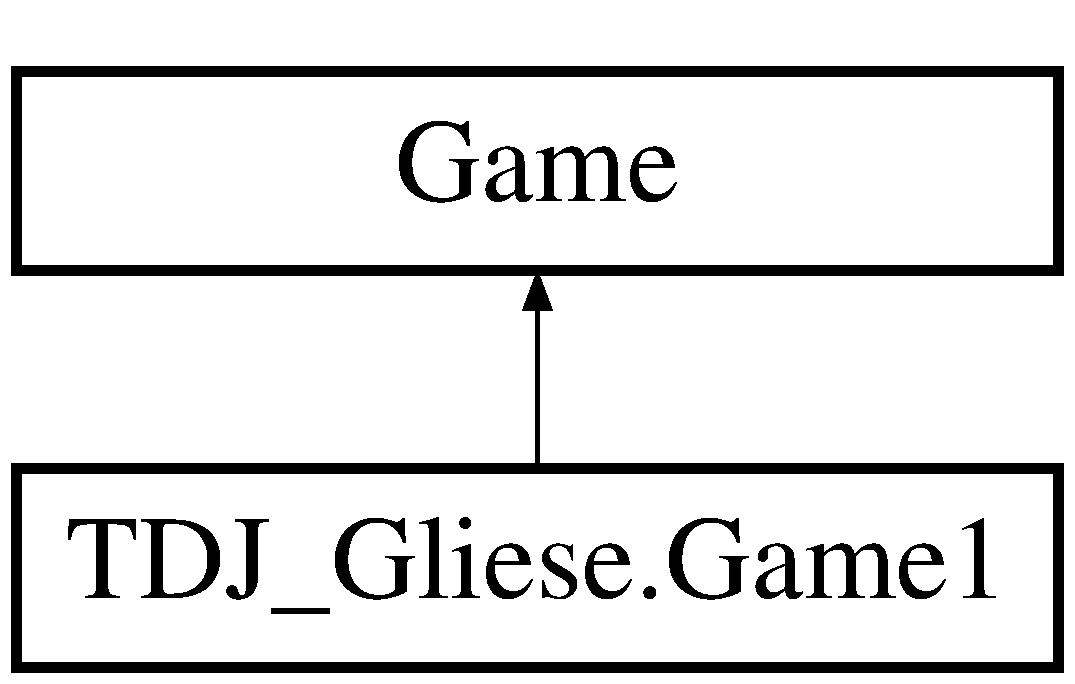
\includegraphics[height=2.000000cm]{class_t_d_j___gliese_1_1_game1}
\end{center}
\end{figure}
\subsection*{Public Member Functions}
\begin{DoxyCompactItemize}
\item 
\hyperlink{class_t_d_j___gliese_1_1_game1_a4ab3d1367aa2bfebb3e81b1d05925cf8}{Game1} ()
\end{DoxyCompactItemize}
\subsection*{Public Attributes}
\begin{DoxyCompactItemize}
\item 
Song \hyperlink{class_t_d_j___gliese_1_1_game1_a62bb1950bf4cc765eabacbe64f80e7ad}{Ketsa}
\item 
Song \hyperlink{class_t_d_j___gliese_1_1_game1_aeeace33dbcd3354a01167dca9e2e7528}{Space\+\_\+\+Back\+Ground\+\_\+\+Music}
\item 
Sprite\+Font \hyperlink{class_t_d_j___gliese_1_1_game1_a382070185267a3730591497cfa98ac96}{font}
\item 
bool \hyperlink{class_t_d_j___gliese_1_1_game1_a9876fddfa3914cd316606efc8638203f}{Goliath\+Locked}
\item 
bool \hyperlink{class_t_d_j___gliese_1_1_game1_ad71bd8c5662aa5e6bee1ecb3b1dc3d7d}{Chaser\+Locked}
\item 
int \hyperlink{class_t_d_j___gliese_1_1_game1_a734bacaf4213efa2a5f597ba23cf6626}{Total\+Score}
\end{DoxyCompactItemize}
\subsection*{Protected Member Functions}
\begin{DoxyCompactItemize}
\item 
override void \hyperlink{class_t_d_j___gliese_1_1_game1_a1960a76d684152d1c60e4f96367701b0}{Initialize} ()
\item 
override void \hyperlink{class_t_d_j___gliese_1_1_game1_ae5cd743cb883778cbf3f0a626e47ef94}{Load\+Content} ()
\item 
override void \hyperlink{class_t_d_j___gliese_1_1_game1_ac3e77e4da26ae3e5a85d4ddca7492819}{Unload\+Content} ()
\item 
override void \hyperlink{class_t_d_j___gliese_1_1_game1_a871390046e9a7a4f8346098eaab3c5b6}{Update} (Game\+Time game\+Time)
\item 
override void \hyperlink{class_t_d_j___gliese_1_1_game1_a5245411dae6b531d02617675fd5d1a8b}{Draw} (Game\+Time game\+Time)
\end{DoxyCompactItemize}


\subsection{Constructor \& Destructor Documentation}
\mbox{\Hypertarget{class_t_d_j___gliese_1_1_game1_a4ab3d1367aa2bfebb3e81b1d05925cf8}\label{class_t_d_j___gliese_1_1_game1_a4ab3d1367aa2bfebb3e81b1d05925cf8}} 
\index{T\+D\+J\+\_\+\+Gliese\+::\+Game1@{T\+D\+J\+\_\+\+Gliese\+::\+Game1}!Game1@{Game1}}
\index{Game1@{Game1}!T\+D\+J\+\_\+\+Gliese\+::\+Game1@{T\+D\+J\+\_\+\+Gliese\+::\+Game1}}
\subsubsection{\texorpdfstring{Game1()}{Game1()}}
{\footnotesize\ttfamily T\+D\+J\+\_\+\+Gliese.\+Game1.\+Game1 (\begin{DoxyParamCaption}{ }\end{DoxyParamCaption})}



\subsection{Member Function Documentation}
\mbox{\Hypertarget{class_t_d_j___gliese_1_1_game1_a5245411dae6b531d02617675fd5d1a8b}\label{class_t_d_j___gliese_1_1_game1_a5245411dae6b531d02617675fd5d1a8b}} 
\index{T\+D\+J\+\_\+\+Gliese\+::\+Game1@{T\+D\+J\+\_\+\+Gliese\+::\+Game1}!Draw@{Draw}}
\index{Draw@{Draw}!T\+D\+J\+\_\+\+Gliese\+::\+Game1@{T\+D\+J\+\_\+\+Gliese\+::\+Game1}}
\subsubsection{\texorpdfstring{Draw()}{Draw()}}
{\footnotesize\ttfamily override void T\+D\+J\+\_\+\+Gliese.\+Game1.\+Draw (\begin{DoxyParamCaption}\item[{Game\+Time}]{game\+Time }\end{DoxyParamCaption})\hspace{0.3cm}{\ttfamily [protected]}}

\mbox{\Hypertarget{class_t_d_j___gliese_1_1_game1_a1960a76d684152d1c60e4f96367701b0}\label{class_t_d_j___gliese_1_1_game1_a1960a76d684152d1c60e4f96367701b0}} 
\index{T\+D\+J\+\_\+\+Gliese\+::\+Game1@{T\+D\+J\+\_\+\+Gliese\+::\+Game1}!Initialize@{Initialize}}
\index{Initialize@{Initialize}!T\+D\+J\+\_\+\+Gliese\+::\+Game1@{T\+D\+J\+\_\+\+Gliese\+::\+Game1}}
\subsubsection{\texorpdfstring{Initialize()}{Initialize()}}
{\footnotesize\ttfamily override void T\+D\+J\+\_\+\+Gliese.\+Game1.\+Initialize (\begin{DoxyParamCaption}{ }\end{DoxyParamCaption})\hspace{0.3cm}{\ttfamily [protected]}}

\mbox{\Hypertarget{class_t_d_j___gliese_1_1_game1_ae5cd743cb883778cbf3f0a626e47ef94}\label{class_t_d_j___gliese_1_1_game1_ae5cd743cb883778cbf3f0a626e47ef94}} 
\index{T\+D\+J\+\_\+\+Gliese\+::\+Game1@{T\+D\+J\+\_\+\+Gliese\+::\+Game1}!Load\+Content@{Load\+Content}}
\index{Load\+Content@{Load\+Content}!T\+D\+J\+\_\+\+Gliese\+::\+Game1@{T\+D\+J\+\_\+\+Gliese\+::\+Game1}}
\subsubsection{\texorpdfstring{Load\+Content()}{LoadContent()}}
{\footnotesize\ttfamily override void T\+D\+J\+\_\+\+Gliese.\+Game1.\+Load\+Content (\begin{DoxyParamCaption}{ }\end{DoxyParamCaption})\hspace{0.3cm}{\ttfamily [protected]}}

\mbox{\Hypertarget{class_t_d_j___gliese_1_1_game1_ac3e77e4da26ae3e5a85d4ddca7492819}\label{class_t_d_j___gliese_1_1_game1_ac3e77e4da26ae3e5a85d4ddca7492819}} 
\index{T\+D\+J\+\_\+\+Gliese\+::\+Game1@{T\+D\+J\+\_\+\+Gliese\+::\+Game1}!Unload\+Content@{Unload\+Content}}
\index{Unload\+Content@{Unload\+Content}!T\+D\+J\+\_\+\+Gliese\+::\+Game1@{T\+D\+J\+\_\+\+Gliese\+::\+Game1}}
\subsubsection{\texorpdfstring{Unload\+Content()}{UnloadContent()}}
{\footnotesize\ttfamily override void T\+D\+J\+\_\+\+Gliese.\+Game1.\+Unload\+Content (\begin{DoxyParamCaption}{ }\end{DoxyParamCaption})\hspace{0.3cm}{\ttfamily [protected]}}

\mbox{\Hypertarget{class_t_d_j___gliese_1_1_game1_a871390046e9a7a4f8346098eaab3c5b6}\label{class_t_d_j___gliese_1_1_game1_a871390046e9a7a4f8346098eaab3c5b6}} 
\index{T\+D\+J\+\_\+\+Gliese\+::\+Game1@{T\+D\+J\+\_\+\+Gliese\+::\+Game1}!Update@{Update}}
\index{Update@{Update}!T\+D\+J\+\_\+\+Gliese\+::\+Game1@{T\+D\+J\+\_\+\+Gliese\+::\+Game1}}
\subsubsection{\texorpdfstring{Update()}{Update()}}
{\footnotesize\ttfamily override void T\+D\+J\+\_\+\+Gliese.\+Game1.\+Update (\begin{DoxyParamCaption}\item[{Game\+Time}]{game\+Time }\end{DoxyParamCaption})\hspace{0.3cm}{\ttfamily [protected]}}



\subsection{Member Data Documentation}
\mbox{\Hypertarget{class_t_d_j___gliese_1_1_game1_ad71bd8c5662aa5e6bee1ecb3b1dc3d7d}\label{class_t_d_j___gliese_1_1_game1_ad71bd8c5662aa5e6bee1ecb3b1dc3d7d}} 
\index{T\+D\+J\+\_\+\+Gliese\+::\+Game1@{T\+D\+J\+\_\+\+Gliese\+::\+Game1}!Chaser\+Locked@{Chaser\+Locked}}
\index{Chaser\+Locked@{Chaser\+Locked}!T\+D\+J\+\_\+\+Gliese\+::\+Game1@{T\+D\+J\+\_\+\+Gliese\+::\+Game1}}
\subsubsection{\texorpdfstring{Chaser\+Locked}{ChaserLocked}}
{\footnotesize\ttfamily bool T\+D\+J\+\_\+\+Gliese.\+Game1.\+Chaser\+Locked}

\mbox{\Hypertarget{class_t_d_j___gliese_1_1_game1_a382070185267a3730591497cfa98ac96}\label{class_t_d_j___gliese_1_1_game1_a382070185267a3730591497cfa98ac96}} 
\index{T\+D\+J\+\_\+\+Gliese\+::\+Game1@{T\+D\+J\+\_\+\+Gliese\+::\+Game1}!font@{font}}
\index{font@{font}!T\+D\+J\+\_\+\+Gliese\+::\+Game1@{T\+D\+J\+\_\+\+Gliese\+::\+Game1}}
\subsubsection{\texorpdfstring{font}{font}}
{\footnotesize\ttfamily Sprite\+Font T\+D\+J\+\_\+\+Gliese.\+Game1.\+font}

\mbox{\Hypertarget{class_t_d_j___gliese_1_1_game1_a9876fddfa3914cd316606efc8638203f}\label{class_t_d_j___gliese_1_1_game1_a9876fddfa3914cd316606efc8638203f}} 
\index{T\+D\+J\+\_\+\+Gliese\+::\+Game1@{T\+D\+J\+\_\+\+Gliese\+::\+Game1}!Goliath\+Locked@{Goliath\+Locked}}
\index{Goliath\+Locked@{Goliath\+Locked}!T\+D\+J\+\_\+\+Gliese\+::\+Game1@{T\+D\+J\+\_\+\+Gliese\+::\+Game1}}
\subsubsection{\texorpdfstring{Goliath\+Locked}{GoliathLocked}}
{\footnotesize\ttfamily bool T\+D\+J\+\_\+\+Gliese.\+Game1.\+Goliath\+Locked}

\mbox{\Hypertarget{class_t_d_j___gliese_1_1_game1_a62bb1950bf4cc765eabacbe64f80e7ad}\label{class_t_d_j___gliese_1_1_game1_a62bb1950bf4cc765eabacbe64f80e7ad}} 
\index{T\+D\+J\+\_\+\+Gliese\+::\+Game1@{T\+D\+J\+\_\+\+Gliese\+::\+Game1}!Ketsa@{Ketsa}}
\index{Ketsa@{Ketsa}!T\+D\+J\+\_\+\+Gliese\+::\+Game1@{T\+D\+J\+\_\+\+Gliese\+::\+Game1}}
\subsubsection{\texorpdfstring{Ketsa}{Ketsa}}
{\footnotesize\ttfamily Song T\+D\+J\+\_\+\+Gliese.\+Game1.\+Ketsa}

\mbox{\Hypertarget{class_t_d_j___gliese_1_1_game1_aeeace33dbcd3354a01167dca9e2e7528}\label{class_t_d_j___gliese_1_1_game1_aeeace33dbcd3354a01167dca9e2e7528}} 
\index{T\+D\+J\+\_\+\+Gliese\+::\+Game1@{T\+D\+J\+\_\+\+Gliese\+::\+Game1}!Space\+\_\+\+Back\+Ground\+\_\+\+Music@{Space\+\_\+\+Back\+Ground\+\_\+\+Music}}
\index{Space\+\_\+\+Back\+Ground\+\_\+\+Music@{Space\+\_\+\+Back\+Ground\+\_\+\+Music}!T\+D\+J\+\_\+\+Gliese\+::\+Game1@{T\+D\+J\+\_\+\+Gliese\+::\+Game1}}
\subsubsection{\texorpdfstring{Space\+\_\+\+Back\+Ground\+\_\+\+Music}{Space\_BackGround\_Music}}
{\footnotesize\ttfamily Song T\+D\+J\+\_\+\+Gliese.\+Game1.\+Space\+\_\+\+Back\+Ground\+\_\+\+Music}

\mbox{\Hypertarget{class_t_d_j___gliese_1_1_game1_a734bacaf4213efa2a5f597ba23cf6626}\label{class_t_d_j___gliese_1_1_game1_a734bacaf4213efa2a5f597ba23cf6626}} 
\index{T\+D\+J\+\_\+\+Gliese\+::\+Game1@{T\+D\+J\+\_\+\+Gliese\+::\+Game1}!Total\+Score@{Total\+Score}}
\index{Total\+Score@{Total\+Score}!T\+D\+J\+\_\+\+Gliese\+::\+Game1@{T\+D\+J\+\_\+\+Gliese\+::\+Game1}}
\subsubsection{\texorpdfstring{Total\+Score}{TotalScore}}
{\footnotesize\ttfamily int T\+D\+J\+\_\+\+Gliese.\+Game1.\+Total\+Score}



The documentation for this class was generated from the following file\+:\begin{DoxyCompactItemize}
\item 
T\+D\+J-\/\+Gliese/\hyperlink{_game1_8cs}{Game1.\+cs}\end{DoxyCompactItemize}

\hypertarget{class_t_d_j___gliese_1_1_l_v_l}{}\section{T\+D\+J\+\_\+\+Gliese.\+L\+VL Class Reference}
\label{class_t_d_j___gliese_1_1_l_v_l}\index{T\+D\+J\+\_\+\+Gliese.\+L\+VL@{T\+D\+J\+\_\+\+Gliese.\+L\+VL}}
\subsection*{Public Member Functions}
\begin{DoxyCompactItemize}
\item 
\hyperlink{class_t_d_j___gliese_1_1_l_v_l_a76589d67b7a7d414ddb3b02fa70f8df7}{L\+VL} (int Width, int Height)
\item 
void \hyperlink{class_t_d_j___gliese_1_1_l_v_l_a05f0bd493f8b55c2cf62ca24bf9ec93e}{Load\+Content\+\_\+\+L\+VL} (Content\+Manager Content)
\item 
void \hyperlink{class_t_d_j___gliese_1_1_l_v_l_aaaea696f38f78962ea2abddcd0ed1f94}{Update\+Content\+\_\+\+L\+VL} (Game\+Time Game\+Time)
\item 
void \hyperlink{class_t_d_j___gliese_1_1_l_v_l_a138ed1b814d02ef00467e81c1abef032}{Draw\+Content\+\_\+\+L\+VL} (Sprite\+Batch Sprite\+Batch, Sprite\+Font Font)
\end{DoxyCompactItemize}
\subsection*{Public Attributes}
\begin{DoxyCompactItemize}
\item 
List$<$ \hyperlink{class_t_d_j___gliese_1_1_enemy_ship}{Enemy\+Ship} $>$ \hyperlink{class_t_d_j___gliese_1_1_l_v_l_a5776de8054cd5e89edde1dc619e7bef3}{Wave1}
\item 
List$<$ \hyperlink{class_t_d_j___gliese_1_1_enemy_ship}{Enemy\+Ship} $>$ \hyperlink{class_t_d_j___gliese_1_1_l_v_l_a3acbe594d5c02022bfd05ce359774cce}{Wave3}
\item 
List$<$ \hyperlink{class_t_d_j___gliese_1_1_enemy_ship}{Enemy\+Ship} $>$ \hyperlink{class_t_d_j___gliese_1_1_l_v_l_a2f82b1c16d7af3fb6f6b80cabc0bcf5b}{Wave4}
\item 
List$<$ \hyperlink{class_t_d_j___gliese_1_1_projectile}{Projectile} $>$ \hyperlink{class_t_d_j___gliese_1_1_l_v_l_aff15a386c2c8a23912cceb3f82b7d4fb}{Enemy\+Projectiles\+List}
\item 
\hyperlink{class_t_d_j___gliese_1_1_enemy_ship}{Enemy\+Ship} \hyperlink{class_t_d_j___gliese_1_1_l_v_l_aaab9650272ee990675e212102bae171f}{B1}
\item 
\hyperlink{class_t_d_j___gliese_1_1_enemy_ship}{Enemy\+Ship} \hyperlink{class_t_d_j___gliese_1_1_l_v_l_a76b806c29150e597473ccd75ec7e83fb}{B2}
\item 
\hyperlink{class_t_d_j___gliese_1_1_enemy_ship}{Enemy\+Ship} \hyperlink{class_t_d_j___gliese_1_1_l_v_l_a86b1b153ab35b94490f5f7cbd234e3f0}{B3}
\item 
\hyperlink{class_t_d_j___gliese_1_1_enemy_ship}{Enemy\+Ship} \hyperlink{class_t_d_j___gliese_1_1_l_v_l_a1cab2204be480949045ae642b53b3ee4}{MB}
\item 
int \hyperlink{class_t_d_j___gliese_1_1_l_v_l_ac5f73d4a33e3f188b277523a65dafcc7}{wave1\+Time}
\item 
int \hyperlink{class_t_d_j___gliese_1_1_l_v_l_ac800c8863c621299f1e3e5e4a9b0da0d}{wave2\+Time}
\item 
int \hyperlink{class_t_d_j___gliese_1_1_l_v_l_a18b306f0c433075602c878fe95b69b66}{wave3\+Time}
\item 
\hyperlink{class_t_d_j___gliese_1_1_power_up}{Power\+Up} \hyperlink{class_t_d_j___gliese_1_1_l_v_l_a94ce5623356b67692c7e4f99309212b5}{L\+V\+Lpowerup}
\item 
int \mbox{[}$\,$\mbox{]} \hyperlink{class_t_d_j___gliese_1_1_l_v_l_aeeee78b5c555039174cb80c85b4b1d2d}{Spawntimes}
\end{DoxyCompactItemize}


\subsection{Constructor \& Destructor Documentation}
\mbox{\Hypertarget{class_t_d_j___gliese_1_1_l_v_l_a76589d67b7a7d414ddb3b02fa70f8df7}\label{class_t_d_j___gliese_1_1_l_v_l_a76589d67b7a7d414ddb3b02fa70f8df7}} 
\index{T\+D\+J\+\_\+\+Gliese\+::\+L\+VL@{T\+D\+J\+\_\+\+Gliese\+::\+L\+VL}!L\+VL@{L\+VL}}
\index{L\+VL@{L\+VL}!T\+D\+J\+\_\+\+Gliese\+::\+L\+VL@{T\+D\+J\+\_\+\+Gliese\+::\+L\+VL}}
\subsubsection{\texorpdfstring{L\+V\+L()}{LVL()}}
{\footnotesize\ttfamily T\+D\+J\+\_\+\+Gliese.\+L\+V\+L.\+L\+VL (\begin{DoxyParamCaption}\item[{int}]{Width,  }\item[{int}]{Height }\end{DoxyParamCaption})}



\subsection{Member Function Documentation}
\mbox{\Hypertarget{class_t_d_j___gliese_1_1_l_v_l_a138ed1b814d02ef00467e81c1abef032}\label{class_t_d_j___gliese_1_1_l_v_l_a138ed1b814d02ef00467e81c1abef032}} 
\index{T\+D\+J\+\_\+\+Gliese\+::\+L\+VL@{T\+D\+J\+\_\+\+Gliese\+::\+L\+VL}!Draw\+Content\+\_\+\+L\+VL@{Draw\+Content\+\_\+\+L\+VL}}
\index{Draw\+Content\+\_\+\+L\+VL@{Draw\+Content\+\_\+\+L\+VL}!T\+D\+J\+\_\+\+Gliese\+::\+L\+VL@{T\+D\+J\+\_\+\+Gliese\+::\+L\+VL}}
\subsubsection{\texorpdfstring{Draw\+Content\+\_\+\+L\+V\+L()}{DrawContent\_LVL()}}
{\footnotesize\ttfamily void T\+D\+J\+\_\+\+Gliese.\+L\+V\+L.\+Draw\+Content\+\_\+\+L\+VL (\begin{DoxyParamCaption}\item[{Sprite\+Batch}]{Sprite\+Batch,  }\item[{Sprite\+Font}]{Font }\end{DoxyParamCaption})}

\mbox{\Hypertarget{class_t_d_j___gliese_1_1_l_v_l_a05f0bd493f8b55c2cf62ca24bf9ec93e}\label{class_t_d_j___gliese_1_1_l_v_l_a05f0bd493f8b55c2cf62ca24bf9ec93e}} 
\index{T\+D\+J\+\_\+\+Gliese\+::\+L\+VL@{T\+D\+J\+\_\+\+Gliese\+::\+L\+VL}!Load\+Content\+\_\+\+L\+VL@{Load\+Content\+\_\+\+L\+VL}}
\index{Load\+Content\+\_\+\+L\+VL@{Load\+Content\+\_\+\+L\+VL}!T\+D\+J\+\_\+\+Gliese\+::\+L\+VL@{T\+D\+J\+\_\+\+Gliese\+::\+L\+VL}}
\subsubsection{\texorpdfstring{Load\+Content\+\_\+\+L\+V\+L()}{LoadContent\_LVL()}}
{\footnotesize\ttfamily void T\+D\+J\+\_\+\+Gliese.\+L\+V\+L.\+Load\+Content\+\_\+\+L\+VL (\begin{DoxyParamCaption}\item[{Content\+Manager}]{Content }\end{DoxyParamCaption})}

\mbox{\Hypertarget{class_t_d_j___gliese_1_1_l_v_l_aaaea696f38f78962ea2abddcd0ed1f94}\label{class_t_d_j___gliese_1_1_l_v_l_aaaea696f38f78962ea2abddcd0ed1f94}} 
\index{T\+D\+J\+\_\+\+Gliese\+::\+L\+VL@{T\+D\+J\+\_\+\+Gliese\+::\+L\+VL}!Update\+Content\+\_\+\+L\+VL@{Update\+Content\+\_\+\+L\+VL}}
\index{Update\+Content\+\_\+\+L\+VL@{Update\+Content\+\_\+\+L\+VL}!T\+D\+J\+\_\+\+Gliese\+::\+L\+VL@{T\+D\+J\+\_\+\+Gliese\+::\+L\+VL}}
\subsubsection{\texorpdfstring{Update\+Content\+\_\+\+L\+V\+L()}{UpdateContent\_LVL()}}
{\footnotesize\ttfamily void T\+D\+J\+\_\+\+Gliese.\+L\+V\+L.\+Update\+Content\+\_\+\+L\+VL (\begin{DoxyParamCaption}\item[{Game\+Time}]{Game\+Time }\end{DoxyParamCaption})}



\subsection{Member Data Documentation}
\mbox{\Hypertarget{class_t_d_j___gliese_1_1_l_v_l_aaab9650272ee990675e212102bae171f}\label{class_t_d_j___gliese_1_1_l_v_l_aaab9650272ee990675e212102bae171f}} 
\index{T\+D\+J\+\_\+\+Gliese\+::\+L\+VL@{T\+D\+J\+\_\+\+Gliese\+::\+L\+VL}!B1@{B1}}
\index{B1@{B1}!T\+D\+J\+\_\+\+Gliese\+::\+L\+VL@{T\+D\+J\+\_\+\+Gliese\+::\+L\+VL}}
\subsubsection{\texorpdfstring{B1}{B1}}
{\footnotesize\ttfamily \hyperlink{class_t_d_j___gliese_1_1_enemy_ship}{Enemy\+Ship} T\+D\+J\+\_\+\+Gliese.\+L\+V\+L.\+B1}

\mbox{\Hypertarget{class_t_d_j___gliese_1_1_l_v_l_a76b806c29150e597473ccd75ec7e83fb}\label{class_t_d_j___gliese_1_1_l_v_l_a76b806c29150e597473ccd75ec7e83fb}} 
\index{T\+D\+J\+\_\+\+Gliese\+::\+L\+VL@{T\+D\+J\+\_\+\+Gliese\+::\+L\+VL}!B2@{B2}}
\index{B2@{B2}!T\+D\+J\+\_\+\+Gliese\+::\+L\+VL@{T\+D\+J\+\_\+\+Gliese\+::\+L\+VL}}
\subsubsection{\texorpdfstring{B2}{B2}}
{\footnotesize\ttfamily \hyperlink{class_t_d_j___gliese_1_1_enemy_ship}{Enemy\+Ship} T\+D\+J\+\_\+\+Gliese.\+L\+V\+L.\+B2}

\mbox{\Hypertarget{class_t_d_j___gliese_1_1_l_v_l_a86b1b153ab35b94490f5f7cbd234e3f0}\label{class_t_d_j___gliese_1_1_l_v_l_a86b1b153ab35b94490f5f7cbd234e3f0}} 
\index{T\+D\+J\+\_\+\+Gliese\+::\+L\+VL@{T\+D\+J\+\_\+\+Gliese\+::\+L\+VL}!B3@{B3}}
\index{B3@{B3}!T\+D\+J\+\_\+\+Gliese\+::\+L\+VL@{T\+D\+J\+\_\+\+Gliese\+::\+L\+VL}}
\subsubsection{\texorpdfstring{B3}{B3}}
{\footnotesize\ttfamily \hyperlink{class_t_d_j___gliese_1_1_enemy_ship}{Enemy\+Ship} T\+D\+J\+\_\+\+Gliese.\+L\+V\+L.\+B3}

\mbox{\Hypertarget{class_t_d_j___gliese_1_1_l_v_l_aff15a386c2c8a23912cceb3f82b7d4fb}\label{class_t_d_j___gliese_1_1_l_v_l_aff15a386c2c8a23912cceb3f82b7d4fb}} 
\index{T\+D\+J\+\_\+\+Gliese\+::\+L\+VL@{T\+D\+J\+\_\+\+Gliese\+::\+L\+VL}!Enemy\+Projectiles\+List@{Enemy\+Projectiles\+List}}
\index{Enemy\+Projectiles\+List@{Enemy\+Projectiles\+List}!T\+D\+J\+\_\+\+Gliese\+::\+L\+VL@{T\+D\+J\+\_\+\+Gliese\+::\+L\+VL}}
\subsubsection{\texorpdfstring{Enemy\+Projectiles\+List}{EnemyProjectilesList}}
{\footnotesize\ttfamily List$<$\hyperlink{class_t_d_j___gliese_1_1_projectile}{Projectile}$>$ T\+D\+J\+\_\+\+Gliese.\+L\+V\+L.\+Enemy\+Projectiles\+List}

\mbox{\Hypertarget{class_t_d_j___gliese_1_1_l_v_l_a94ce5623356b67692c7e4f99309212b5}\label{class_t_d_j___gliese_1_1_l_v_l_a94ce5623356b67692c7e4f99309212b5}} 
\index{T\+D\+J\+\_\+\+Gliese\+::\+L\+VL@{T\+D\+J\+\_\+\+Gliese\+::\+L\+VL}!L\+V\+Lpowerup@{L\+V\+Lpowerup}}
\index{L\+V\+Lpowerup@{L\+V\+Lpowerup}!T\+D\+J\+\_\+\+Gliese\+::\+L\+VL@{T\+D\+J\+\_\+\+Gliese\+::\+L\+VL}}
\subsubsection{\texorpdfstring{L\+V\+Lpowerup}{LVLpowerup}}
{\footnotesize\ttfamily \hyperlink{class_t_d_j___gliese_1_1_power_up}{Power\+Up} T\+D\+J\+\_\+\+Gliese.\+L\+V\+L.\+L\+V\+Lpowerup}

\mbox{\Hypertarget{class_t_d_j___gliese_1_1_l_v_l_a1cab2204be480949045ae642b53b3ee4}\label{class_t_d_j___gliese_1_1_l_v_l_a1cab2204be480949045ae642b53b3ee4}} 
\index{T\+D\+J\+\_\+\+Gliese\+::\+L\+VL@{T\+D\+J\+\_\+\+Gliese\+::\+L\+VL}!MB@{MB}}
\index{MB@{MB}!T\+D\+J\+\_\+\+Gliese\+::\+L\+VL@{T\+D\+J\+\_\+\+Gliese\+::\+L\+VL}}
\subsubsection{\texorpdfstring{MB}{MB}}
{\footnotesize\ttfamily \hyperlink{class_t_d_j___gliese_1_1_enemy_ship}{Enemy\+Ship} T\+D\+J\+\_\+\+Gliese.\+L\+V\+L.\+MB}

\mbox{\Hypertarget{class_t_d_j___gliese_1_1_l_v_l_aeeee78b5c555039174cb80c85b4b1d2d}\label{class_t_d_j___gliese_1_1_l_v_l_aeeee78b5c555039174cb80c85b4b1d2d}} 
\index{T\+D\+J\+\_\+\+Gliese\+::\+L\+VL@{T\+D\+J\+\_\+\+Gliese\+::\+L\+VL}!Spawntimes@{Spawntimes}}
\index{Spawntimes@{Spawntimes}!T\+D\+J\+\_\+\+Gliese\+::\+L\+VL@{T\+D\+J\+\_\+\+Gliese\+::\+L\+VL}}
\subsubsection{\texorpdfstring{Spawntimes}{Spawntimes}}
{\footnotesize\ttfamily int \mbox{[}$\,$\mbox{]} T\+D\+J\+\_\+\+Gliese.\+L\+V\+L.\+Spawntimes}

\mbox{\Hypertarget{class_t_d_j___gliese_1_1_l_v_l_a5776de8054cd5e89edde1dc619e7bef3}\label{class_t_d_j___gliese_1_1_l_v_l_a5776de8054cd5e89edde1dc619e7bef3}} 
\index{T\+D\+J\+\_\+\+Gliese\+::\+L\+VL@{T\+D\+J\+\_\+\+Gliese\+::\+L\+VL}!Wave1@{Wave1}}
\index{Wave1@{Wave1}!T\+D\+J\+\_\+\+Gliese\+::\+L\+VL@{T\+D\+J\+\_\+\+Gliese\+::\+L\+VL}}
\subsubsection{\texorpdfstring{Wave1}{Wave1}}
{\footnotesize\ttfamily List$<$\hyperlink{class_t_d_j___gliese_1_1_enemy_ship}{Enemy\+Ship}$>$ T\+D\+J\+\_\+\+Gliese.\+L\+V\+L.\+Wave1}

\mbox{\Hypertarget{class_t_d_j___gliese_1_1_l_v_l_ac5f73d4a33e3f188b277523a65dafcc7}\label{class_t_d_j___gliese_1_1_l_v_l_ac5f73d4a33e3f188b277523a65dafcc7}} 
\index{T\+D\+J\+\_\+\+Gliese\+::\+L\+VL@{T\+D\+J\+\_\+\+Gliese\+::\+L\+VL}!wave1\+Time@{wave1\+Time}}
\index{wave1\+Time@{wave1\+Time}!T\+D\+J\+\_\+\+Gliese\+::\+L\+VL@{T\+D\+J\+\_\+\+Gliese\+::\+L\+VL}}
\subsubsection{\texorpdfstring{wave1\+Time}{wave1Time}}
{\footnotesize\ttfamily int T\+D\+J\+\_\+\+Gliese.\+L\+V\+L.\+wave1\+Time}

\mbox{\Hypertarget{class_t_d_j___gliese_1_1_l_v_l_ac800c8863c621299f1e3e5e4a9b0da0d}\label{class_t_d_j___gliese_1_1_l_v_l_ac800c8863c621299f1e3e5e4a9b0da0d}} 
\index{T\+D\+J\+\_\+\+Gliese\+::\+L\+VL@{T\+D\+J\+\_\+\+Gliese\+::\+L\+VL}!wave2\+Time@{wave2\+Time}}
\index{wave2\+Time@{wave2\+Time}!T\+D\+J\+\_\+\+Gliese\+::\+L\+VL@{T\+D\+J\+\_\+\+Gliese\+::\+L\+VL}}
\subsubsection{\texorpdfstring{wave2\+Time}{wave2Time}}
{\footnotesize\ttfamily int T\+D\+J\+\_\+\+Gliese.\+L\+V\+L.\+wave2\+Time}

\mbox{\Hypertarget{class_t_d_j___gliese_1_1_l_v_l_a3acbe594d5c02022bfd05ce359774cce}\label{class_t_d_j___gliese_1_1_l_v_l_a3acbe594d5c02022bfd05ce359774cce}} 
\index{T\+D\+J\+\_\+\+Gliese\+::\+L\+VL@{T\+D\+J\+\_\+\+Gliese\+::\+L\+VL}!Wave3@{Wave3}}
\index{Wave3@{Wave3}!T\+D\+J\+\_\+\+Gliese\+::\+L\+VL@{T\+D\+J\+\_\+\+Gliese\+::\+L\+VL}}
\subsubsection{\texorpdfstring{Wave3}{Wave3}}
{\footnotesize\ttfamily List$<$\hyperlink{class_t_d_j___gliese_1_1_enemy_ship}{Enemy\+Ship}$>$ T\+D\+J\+\_\+\+Gliese.\+L\+V\+L.\+Wave3}

\mbox{\Hypertarget{class_t_d_j___gliese_1_1_l_v_l_a18b306f0c433075602c878fe95b69b66}\label{class_t_d_j___gliese_1_1_l_v_l_a18b306f0c433075602c878fe95b69b66}} 
\index{T\+D\+J\+\_\+\+Gliese\+::\+L\+VL@{T\+D\+J\+\_\+\+Gliese\+::\+L\+VL}!wave3\+Time@{wave3\+Time}}
\index{wave3\+Time@{wave3\+Time}!T\+D\+J\+\_\+\+Gliese\+::\+L\+VL@{T\+D\+J\+\_\+\+Gliese\+::\+L\+VL}}
\subsubsection{\texorpdfstring{wave3\+Time}{wave3Time}}
{\footnotesize\ttfamily int T\+D\+J\+\_\+\+Gliese.\+L\+V\+L.\+wave3\+Time}

\mbox{\Hypertarget{class_t_d_j___gliese_1_1_l_v_l_a2f82b1c16d7af3fb6f6b80cabc0bcf5b}\label{class_t_d_j___gliese_1_1_l_v_l_a2f82b1c16d7af3fb6f6b80cabc0bcf5b}} 
\index{T\+D\+J\+\_\+\+Gliese\+::\+L\+VL@{T\+D\+J\+\_\+\+Gliese\+::\+L\+VL}!Wave4@{Wave4}}
\index{Wave4@{Wave4}!T\+D\+J\+\_\+\+Gliese\+::\+L\+VL@{T\+D\+J\+\_\+\+Gliese\+::\+L\+VL}}
\subsubsection{\texorpdfstring{Wave4}{Wave4}}
{\footnotesize\ttfamily List$<$\hyperlink{class_t_d_j___gliese_1_1_enemy_ship}{Enemy\+Ship}$>$ T\+D\+J\+\_\+\+Gliese.\+L\+V\+L.\+Wave4}



The documentation for this class was generated from the following file\+:\begin{DoxyCompactItemize}
\item 
T\+D\+J-\/\+Gliese/\hyperlink{_l_v_l_8cs}{L\+V\+L.\+cs}\end{DoxyCompactItemize}

\hypertarget{class_t_d_j___gliese_1_1_pause_menu}{}\section{T\+D\+J\+\_\+\+Gliese.\+Pause\+Menu Class Reference}
\label{class_t_d_j___gliese_1_1_pause_menu}\index{T\+D\+J\+\_\+\+Gliese.\+Pause\+Menu@{T\+D\+J\+\_\+\+Gliese.\+Pause\+Menu}}


The documentation for this class was generated from the following file\+:\begin{DoxyCompactItemize}
\item 
T\+D\+J-\/\+Gliese/\hyperlink{_pause_menu_8cs}{Pause\+Menu.\+cs}\end{DoxyCompactItemize}

\hypertarget{class_t_d_j___gliese_1_1_power_up}{}\section{T\+D\+J\+\_\+\+Gliese.\+Power\+Up Class Reference}
\label{class_t_d_j___gliese_1_1_power_up}\index{T\+D\+J\+\_\+\+Gliese.\+Power\+Up@{T\+D\+J\+\_\+\+Gliese.\+Power\+Up}}
\subsection*{Public Member Functions}
\begin{DoxyCompactItemize}
\item 
\hyperlink{class_t_d_j___gliese_1_1_power_up_af748c62a6501f8fedcf130ac1c32834f}{Power\+Up} (Texture2D Enemy, int Width, int Height)
\item 
void \hyperlink{class_t_d_j___gliese_1_1_power_up_a2b15d72dcb58cbc354e386664b7bc8e0}{Update} (Game\+Time gametime)
\item 
void \hyperlink{class_t_d_j___gliese_1_1_power_up_ac46db01ba96c843eeeabfa649bd09c12}{Draw} (Sprite\+Batch spritebatch)
\end{DoxyCompactItemize}
\subsection*{Public Attributes}
\begin{DoxyCompactItemize}
\item 
Texture2D \hyperlink{class_t_d_j___gliese_1_1_power_up_a574052ea0c87264da315ee0e3f9259c3}{texture}
\item 
bool \hyperlink{class_t_d_j___gliese_1_1_power_up_af4ff6682145e48f9a65c9905ceaf6d4f}{Isdestroyed}
\item 
Rectangle \hyperlink{class_t_d_j___gliese_1_1_power_up_a0d85f59ad9a8c0150ffb5ce36764a69d}{Colision\+Box}
\end{DoxyCompactItemize}


\subsection{Constructor \& Destructor Documentation}
\mbox{\Hypertarget{class_t_d_j___gliese_1_1_power_up_af748c62a6501f8fedcf130ac1c32834f}\label{class_t_d_j___gliese_1_1_power_up_af748c62a6501f8fedcf130ac1c32834f}} 
\index{T\+D\+J\+\_\+\+Gliese\+::\+Power\+Up@{T\+D\+J\+\_\+\+Gliese\+::\+Power\+Up}!Power\+Up@{Power\+Up}}
\index{Power\+Up@{Power\+Up}!T\+D\+J\+\_\+\+Gliese\+::\+Power\+Up@{T\+D\+J\+\_\+\+Gliese\+::\+Power\+Up}}
\subsubsection{\texorpdfstring{Power\+Up()}{PowerUp()}}
{\footnotesize\ttfamily T\+D\+J\+\_\+\+Gliese.\+Power\+Up.\+Power\+Up (\begin{DoxyParamCaption}\item[{Texture2D}]{Enemy,  }\item[{int}]{Width,  }\item[{int}]{Height }\end{DoxyParamCaption})}



\subsection{Member Function Documentation}
\mbox{\Hypertarget{class_t_d_j___gliese_1_1_power_up_ac46db01ba96c843eeeabfa649bd09c12}\label{class_t_d_j___gliese_1_1_power_up_ac46db01ba96c843eeeabfa649bd09c12}} 
\index{T\+D\+J\+\_\+\+Gliese\+::\+Power\+Up@{T\+D\+J\+\_\+\+Gliese\+::\+Power\+Up}!Draw@{Draw}}
\index{Draw@{Draw}!T\+D\+J\+\_\+\+Gliese\+::\+Power\+Up@{T\+D\+J\+\_\+\+Gliese\+::\+Power\+Up}}
\subsubsection{\texorpdfstring{Draw()}{Draw()}}
{\footnotesize\ttfamily void T\+D\+J\+\_\+\+Gliese.\+Power\+Up.\+Draw (\begin{DoxyParamCaption}\item[{Sprite\+Batch}]{spritebatch }\end{DoxyParamCaption})}

\mbox{\Hypertarget{class_t_d_j___gliese_1_1_power_up_a2b15d72dcb58cbc354e386664b7bc8e0}\label{class_t_d_j___gliese_1_1_power_up_a2b15d72dcb58cbc354e386664b7bc8e0}} 
\index{T\+D\+J\+\_\+\+Gliese\+::\+Power\+Up@{T\+D\+J\+\_\+\+Gliese\+::\+Power\+Up}!Update@{Update}}
\index{Update@{Update}!T\+D\+J\+\_\+\+Gliese\+::\+Power\+Up@{T\+D\+J\+\_\+\+Gliese\+::\+Power\+Up}}
\subsubsection{\texorpdfstring{Update()}{Update()}}
{\footnotesize\ttfamily void T\+D\+J\+\_\+\+Gliese.\+Power\+Up.\+Update (\begin{DoxyParamCaption}\item[{Game\+Time}]{gametime }\end{DoxyParamCaption})}



\subsection{Member Data Documentation}
\mbox{\Hypertarget{class_t_d_j___gliese_1_1_power_up_a0d85f59ad9a8c0150ffb5ce36764a69d}\label{class_t_d_j___gliese_1_1_power_up_a0d85f59ad9a8c0150ffb5ce36764a69d}} 
\index{T\+D\+J\+\_\+\+Gliese\+::\+Power\+Up@{T\+D\+J\+\_\+\+Gliese\+::\+Power\+Up}!Colision\+Box@{Colision\+Box}}
\index{Colision\+Box@{Colision\+Box}!T\+D\+J\+\_\+\+Gliese\+::\+Power\+Up@{T\+D\+J\+\_\+\+Gliese\+::\+Power\+Up}}
\subsubsection{\texorpdfstring{Colision\+Box}{ColisionBox}}
{\footnotesize\ttfamily Rectangle T\+D\+J\+\_\+\+Gliese.\+Power\+Up.\+Colision\+Box}

\mbox{\Hypertarget{class_t_d_j___gliese_1_1_power_up_af4ff6682145e48f9a65c9905ceaf6d4f}\label{class_t_d_j___gliese_1_1_power_up_af4ff6682145e48f9a65c9905ceaf6d4f}} 
\index{T\+D\+J\+\_\+\+Gliese\+::\+Power\+Up@{T\+D\+J\+\_\+\+Gliese\+::\+Power\+Up}!Isdestroyed@{Isdestroyed}}
\index{Isdestroyed@{Isdestroyed}!T\+D\+J\+\_\+\+Gliese\+::\+Power\+Up@{T\+D\+J\+\_\+\+Gliese\+::\+Power\+Up}}
\subsubsection{\texorpdfstring{Isdestroyed}{Isdestroyed}}
{\footnotesize\ttfamily bool T\+D\+J\+\_\+\+Gliese.\+Power\+Up.\+Isdestroyed}

\mbox{\Hypertarget{class_t_d_j___gliese_1_1_power_up_a574052ea0c87264da315ee0e3f9259c3}\label{class_t_d_j___gliese_1_1_power_up_a574052ea0c87264da315ee0e3f9259c3}} 
\index{T\+D\+J\+\_\+\+Gliese\+::\+Power\+Up@{T\+D\+J\+\_\+\+Gliese\+::\+Power\+Up}!texture@{texture}}
\index{texture@{texture}!T\+D\+J\+\_\+\+Gliese\+::\+Power\+Up@{T\+D\+J\+\_\+\+Gliese\+::\+Power\+Up}}
\subsubsection{\texorpdfstring{texture}{texture}}
{\footnotesize\ttfamily Texture2D T\+D\+J\+\_\+\+Gliese.\+Power\+Up.\+texture}



The documentation for this class was generated from the following file\+:\begin{DoxyCompactItemize}
\item 
T\+D\+J-\/\+Gliese/\hyperlink{_power_up_8cs}{Power\+Up.\+cs}\end{DoxyCompactItemize}

\hypertarget{class_t_d_j___gliese_1_1_projectile}{}\section{T\+D\+J\+\_\+\+Gliese.\+Projectile Class Reference}
\label{class_t_d_j___gliese_1_1_projectile}\index{T\+D\+J\+\_\+\+Gliese.\+Projectile@{T\+D\+J\+\_\+\+Gliese.\+Projectile}}
\subsection*{Public Member Functions}
\begin{DoxyCompactItemize}
\item 
\hyperlink{class_t_d_j___gliese_1_1_projectile_a836d7c7156fee64079dad6fe0a313fe9}{Projectile} (Texture2D texture)
\item 
void \hyperlink{class_t_d_j___gliese_1_1_projectile_ad650f132cf8f79674ea4beafb8a62938}{Draw\+\_\+\+Projectile} (Sprite\+Batch spritebatch)
\end{DoxyCompactItemize}
\subsection*{Public Attributes}
\begin{DoxyCompactItemize}
\item 
Texture2D \hyperlink{class_t_d_j___gliese_1_1_projectile_a11ccc3fc13f12c356a855dc14d716204}{Projectile\+\_\+\+Image}
\item 
Rectangle \hyperlink{class_t_d_j___gliese_1_1_projectile_a73e50d3e692c5829e849d7a6d9e2ef25}{Projectile\+\_\+\+Colision\+Box}
\item 
bool \hyperlink{class_t_d_j___gliese_1_1_projectile_a80257c9ac2eb31516f0bfeaa560bfd27}{isvisible}
\item 
int \hyperlink{class_t_d_j___gliese_1_1_projectile_aba7ed8680effd7857fb6ca5ea86fd769}{Shoot\+Speed}
\item 
int \hyperlink{class_t_d_j___gliese_1_1_projectile_a856e754a7b21dff3d22fe4ac77a67ae1}{Projectile\+Damage}
\end{DoxyCompactItemize}


\subsection{Constructor \& Destructor Documentation}
\mbox{\Hypertarget{class_t_d_j___gliese_1_1_projectile_a836d7c7156fee64079dad6fe0a313fe9}\label{class_t_d_j___gliese_1_1_projectile_a836d7c7156fee64079dad6fe0a313fe9}} 
\index{T\+D\+J\+\_\+\+Gliese\+::\+Projectile@{T\+D\+J\+\_\+\+Gliese\+::\+Projectile}!Projectile@{Projectile}}
\index{Projectile@{Projectile}!T\+D\+J\+\_\+\+Gliese\+::\+Projectile@{T\+D\+J\+\_\+\+Gliese\+::\+Projectile}}
\subsubsection{\texorpdfstring{Projectile()}{Projectile()}}
{\footnotesize\ttfamily T\+D\+J\+\_\+\+Gliese.\+Projectile.\+Projectile (\begin{DoxyParamCaption}\item[{Texture2D}]{texture }\end{DoxyParamCaption})}



\subsection{Member Function Documentation}
\mbox{\Hypertarget{class_t_d_j___gliese_1_1_projectile_ad650f132cf8f79674ea4beafb8a62938}\label{class_t_d_j___gliese_1_1_projectile_ad650f132cf8f79674ea4beafb8a62938}} 
\index{T\+D\+J\+\_\+\+Gliese\+::\+Projectile@{T\+D\+J\+\_\+\+Gliese\+::\+Projectile}!Draw\+\_\+\+Projectile@{Draw\+\_\+\+Projectile}}
\index{Draw\+\_\+\+Projectile@{Draw\+\_\+\+Projectile}!T\+D\+J\+\_\+\+Gliese\+::\+Projectile@{T\+D\+J\+\_\+\+Gliese\+::\+Projectile}}
\subsubsection{\texorpdfstring{Draw\+\_\+\+Projectile()}{Draw\_Projectile()}}
{\footnotesize\ttfamily void T\+D\+J\+\_\+\+Gliese.\+Projectile.\+Draw\+\_\+\+Projectile (\begin{DoxyParamCaption}\item[{Sprite\+Batch}]{spritebatch }\end{DoxyParamCaption})}



\subsection{Member Data Documentation}
\mbox{\Hypertarget{class_t_d_j___gliese_1_1_projectile_a80257c9ac2eb31516f0bfeaa560bfd27}\label{class_t_d_j___gliese_1_1_projectile_a80257c9ac2eb31516f0bfeaa560bfd27}} 
\index{T\+D\+J\+\_\+\+Gliese\+::\+Projectile@{T\+D\+J\+\_\+\+Gliese\+::\+Projectile}!isvisible@{isvisible}}
\index{isvisible@{isvisible}!T\+D\+J\+\_\+\+Gliese\+::\+Projectile@{T\+D\+J\+\_\+\+Gliese\+::\+Projectile}}
\subsubsection{\texorpdfstring{isvisible}{isvisible}}
{\footnotesize\ttfamily bool T\+D\+J\+\_\+\+Gliese.\+Projectile.\+isvisible}

\mbox{\Hypertarget{class_t_d_j___gliese_1_1_projectile_a73e50d3e692c5829e849d7a6d9e2ef25}\label{class_t_d_j___gliese_1_1_projectile_a73e50d3e692c5829e849d7a6d9e2ef25}} 
\index{T\+D\+J\+\_\+\+Gliese\+::\+Projectile@{T\+D\+J\+\_\+\+Gliese\+::\+Projectile}!Projectile\+\_\+\+Colision\+Box@{Projectile\+\_\+\+Colision\+Box}}
\index{Projectile\+\_\+\+Colision\+Box@{Projectile\+\_\+\+Colision\+Box}!T\+D\+J\+\_\+\+Gliese\+::\+Projectile@{T\+D\+J\+\_\+\+Gliese\+::\+Projectile}}
\subsubsection{\texorpdfstring{Projectile\+\_\+\+Colision\+Box}{Projectile\_ColisionBox}}
{\footnotesize\ttfamily Rectangle T\+D\+J\+\_\+\+Gliese.\+Projectile.\+Projectile\+\_\+\+Colision\+Box}

\mbox{\Hypertarget{class_t_d_j___gliese_1_1_projectile_a11ccc3fc13f12c356a855dc14d716204}\label{class_t_d_j___gliese_1_1_projectile_a11ccc3fc13f12c356a855dc14d716204}} 
\index{T\+D\+J\+\_\+\+Gliese\+::\+Projectile@{T\+D\+J\+\_\+\+Gliese\+::\+Projectile}!Projectile\+\_\+\+Image@{Projectile\+\_\+\+Image}}
\index{Projectile\+\_\+\+Image@{Projectile\+\_\+\+Image}!T\+D\+J\+\_\+\+Gliese\+::\+Projectile@{T\+D\+J\+\_\+\+Gliese\+::\+Projectile}}
\subsubsection{\texorpdfstring{Projectile\+\_\+\+Image}{Projectile\_Image}}
{\footnotesize\ttfamily Texture2D T\+D\+J\+\_\+\+Gliese.\+Projectile.\+Projectile\+\_\+\+Image}

\mbox{\Hypertarget{class_t_d_j___gliese_1_1_projectile_a856e754a7b21dff3d22fe4ac77a67ae1}\label{class_t_d_j___gliese_1_1_projectile_a856e754a7b21dff3d22fe4ac77a67ae1}} 
\index{T\+D\+J\+\_\+\+Gliese\+::\+Projectile@{T\+D\+J\+\_\+\+Gliese\+::\+Projectile}!Projectile\+Damage@{Projectile\+Damage}}
\index{Projectile\+Damage@{Projectile\+Damage}!T\+D\+J\+\_\+\+Gliese\+::\+Projectile@{T\+D\+J\+\_\+\+Gliese\+::\+Projectile}}
\subsubsection{\texorpdfstring{Projectile\+Damage}{ProjectileDamage}}
{\footnotesize\ttfamily int T\+D\+J\+\_\+\+Gliese.\+Projectile.\+Projectile\+Damage}

\mbox{\Hypertarget{class_t_d_j___gliese_1_1_projectile_aba7ed8680effd7857fb6ca5ea86fd769}\label{class_t_d_j___gliese_1_1_projectile_aba7ed8680effd7857fb6ca5ea86fd769}} 
\index{T\+D\+J\+\_\+\+Gliese\+::\+Projectile@{T\+D\+J\+\_\+\+Gliese\+::\+Projectile}!Shoot\+Speed@{Shoot\+Speed}}
\index{Shoot\+Speed@{Shoot\+Speed}!T\+D\+J\+\_\+\+Gliese\+::\+Projectile@{T\+D\+J\+\_\+\+Gliese\+::\+Projectile}}
\subsubsection{\texorpdfstring{Shoot\+Speed}{ShootSpeed}}
{\footnotesize\ttfamily int T\+D\+J\+\_\+\+Gliese.\+Projectile.\+Shoot\+Speed}



The documentation for this class was generated from the following file\+:\begin{DoxyCompactItemize}
\item 
T\+D\+J-\/\+Gliese/\hyperlink{_projectile_8cs}{Projectile.\+cs}\end{DoxyCompactItemize}

\hypertarget{class_t_d_j___gliese_1_1_ship}{}\section{T\+D\+J\+\_\+\+Gliese.\+Ship Class Reference}
\label{class_t_d_j___gliese_1_1_ship}\index{T\+D\+J\+\_\+\+Gliese.\+Ship@{T\+D\+J\+\_\+\+Gliese.\+Ship}}
\subsection*{Public Member Functions}
\begin{DoxyCompactItemize}
\item 
\hyperlink{class_t_d_j___gliese_1_1_ship_ac6484a415970f8daa937d940aef48a57}{Ship} (int Tier, int Width, int Height)
\item 
void \hyperlink{class_t_d_j___gliese_1_1_ship_a19964ca50d3961a08f414d8deca7291c}{Load\+\_\+content\+\_\+\+Ship} (Content\+Manager Content)
\item 
void \hyperlink{class_t_d_j___gliese_1_1_ship_a363f5776505f9baf33ae8651547f6ff8}{Update\+\_\+\+Tier} ()
\item 
void \hyperlink{class_t_d_j___gliese_1_1_ship_a30aa20d3d1fbb797eedb19deffd5da72}{Update\+\_\+\+Ship} (Game\+Time Gametime)
\item 
void \hyperlink{class_t_d_j___gliese_1_1_ship_ade17691846d292b3e780c5667a9cc5ee}{Is\+\_\+ship\+\_\+\+Coliding} (List$<$ \hyperlink{class_t_d_j___gliese_1_1_enemy_ship}{Enemy\+Ship} $>$ Enemylist)
\item 
void \hyperlink{class_t_d_j___gliese_1_1_ship_aa2cb84ed2f07f47eadc04e86a0fb77c1}{Draw\+\_\+\+Ship} (Sprite\+Batch spritebatch, Sprite\+Font Font)
\end{DoxyCompactItemize}
\subsection*{Public Attributes}
\begin{DoxyCompactItemize}
\item 
Rectangle \hyperlink{class_t_d_j___gliese_1_1_ship_ac94ff68060753b5a57183a414e10198c}{Ship\+\_\+\+Colision\+Box}
\item 
bool \hyperlink{class_t_d_j___gliese_1_1_ship_ab04d95577b2e9d59038beb15d4c44517}{Ship\+\_\+\+Is\+\_\+\+Destructed}
\item 
bool \hyperlink{class_t_d_j___gliese_1_1_ship_a6fd70556744e25e1743cc27f566018cd}{isbeinghit}
\item 
int \hyperlink{class_t_d_j___gliese_1_1_ship_a944a147b9a2e0391499617014f1a79a9}{Kind\+\_\+\+Of\+\_\+\+Power\+\_\+\+Up}
\item 
int \hyperlink{class_t_d_j___gliese_1_1_ship_a5a045b903027b805f2bf6893cce33784}{Avaliable\+Points}
\item 
int \hyperlink{class_t_d_j___gliese_1_1_ship_aed7ff40de6c54938a7589595379b1195}{Ship\+\_\+\+Speed\+\_\+\+P\+TS}
\item 
int \hyperlink{class_t_d_j___gliese_1_1_ship_a12a03cfeace42db0d257ce4f75c456f6}{Ship\+\_\+\+Endurance\+\_\+\+P\+TS}
\item 
int \hyperlink{class_t_d_j___gliese_1_1_ship_a145313c1949b730fc835fd7325b375d9}{Ship\+\_\+\+Total\+\_\+\+H\+P\+\_\+\+P\+TS}
\item 
int \hyperlink{class_t_d_j___gliese_1_1_ship_abb4db4b5321a9cf19f9dbedc92a34113}{Ship\+\_\+\+Shooting\+\_\+\+Speed\+\_\+\+P\+TS}
\item 
int \hyperlink{class_t_d_j___gliese_1_1_ship_adc2a27973f237ed489ce8002b87055f4}{Projectile\+\_\+\+Damage\+\_\+\+P\+TS}
\item 
int \hyperlink{class_t_d_j___gliese_1_1_ship_a3c547516f746218184f5752bb2126ac5}{Ship\+\_\+\+Tier}
\item 
int \hyperlink{class_t_d_j___gliese_1_1_ship_a4dfc99b5768e2c500e2f530ce65c3a65}{Ship\+\_\+\+Speed}
\item 
int \hyperlink{class_t_d_j___gliese_1_1_ship_a714c6a21bfad19da1f4f8ab388b0793c}{Projectile\+\_\+\+Delay}
\item 
Texture2D \hyperlink{class_t_d_j___gliese_1_1_ship_a7c579568b281500132258c25b8dc41f6}{Projectile\+\_\+\+Image}
\item 
List$<$ \hyperlink{class_t_d_j___gliese_1_1_projectile}{Projectile} $>$ \hyperlink{class_t_d_j___gliese_1_1_ship_aa4dd7af04e2eba843ee65a5890a6f683}{Projectiles\+\_\+\+List}
\item 
int \hyperlink{class_t_d_j___gliese_1_1_ship_a9b8a46c11a735285804f87466ca1641c}{score}
\item 
List$<$ \hyperlink{class_t_d_j___gliese_1_1_content_1_1_boom}{Boom} $>$ \hyperlink{class_t_d_j___gliese_1_1_ship_a88182145d60126a7a22abfe10232b25d}{Explosions\+List}
\end{DoxyCompactItemize}


\subsection{Constructor \& Destructor Documentation}
\mbox{\Hypertarget{class_t_d_j___gliese_1_1_ship_ac6484a415970f8daa937d940aef48a57}\label{class_t_d_j___gliese_1_1_ship_ac6484a415970f8daa937d940aef48a57}} 
\index{T\+D\+J\+\_\+\+Gliese\+::\+Ship@{T\+D\+J\+\_\+\+Gliese\+::\+Ship}!Ship@{Ship}}
\index{Ship@{Ship}!T\+D\+J\+\_\+\+Gliese\+::\+Ship@{T\+D\+J\+\_\+\+Gliese\+::\+Ship}}
\subsubsection{\texorpdfstring{Ship()}{Ship()}}
{\footnotesize\ttfamily T\+D\+J\+\_\+\+Gliese.\+Ship.\+Ship (\begin{DoxyParamCaption}\item[{int}]{Tier,  }\item[{int}]{Width,  }\item[{int}]{Height }\end{DoxyParamCaption})}



\subsection{Member Function Documentation}
\mbox{\Hypertarget{class_t_d_j___gliese_1_1_ship_aa2cb84ed2f07f47eadc04e86a0fb77c1}\label{class_t_d_j___gliese_1_1_ship_aa2cb84ed2f07f47eadc04e86a0fb77c1}} 
\index{T\+D\+J\+\_\+\+Gliese\+::\+Ship@{T\+D\+J\+\_\+\+Gliese\+::\+Ship}!Draw\+\_\+\+Ship@{Draw\+\_\+\+Ship}}
\index{Draw\+\_\+\+Ship@{Draw\+\_\+\+Ship}!T\+D\+J\+\_\+\+Gliese\+::\+Ship@{T\+D\+J\+\_\+\+Gliese\+::\+Ship}}
\subsubsection{\texorpdfstring{Draw\+\_\+\+Ship()}{Draw\_Ship()}}
{\footnotesize\ttfamily void T\+D\+J\+\_\+\+Gliese.\+Ship.\+Draw\+\_\+\+Ship (\begin{DoxyParamCaption}\item[{Sprite\+Batch}]{spritebatch,  }\item[{Sprite\+Font}]{Font }\end{DoxyParamCaption})}

\mbox{\Hypertarget{class_t_d_j___gliese_1_1_ship_ade17691846d292b3e780c5667a9cc5ee}\label{class_t_d_j___gliese_1_1_ship_ade17691846d292b3e780c5667a9cc5ee}} 
\index{T\+D\+J\+\_\+\+Gliese\+::\+Ship@{T\+D\+J\+\_\+\+Gliese\+::\+Ship}!Is\+\_\+ship\+\_\+\+Coliding@{Is\+\_\+ship\+\_\+\+Coliding}}
\index{Is\+\_\+ship\+\_\+\+Coliding@{Is\+\_\+ship\+\_\+\+Coliding}!T\+D\+J\+\_\+\+Gliese\+::\+Ship@{T\+D\+J\+\_\+\+Gliese\+::\+Ship}}
\subsubsection{\texorpdfstring{Is\+\_\+ship\+\_\+\+Coliding()}{Is\_ship\_Coliding()}}
{\footnotesize\ttfamily void T\+D\+J\+\_\+\+Gliese.\+Ship.\+Is\+\_\+ship\+\_\+\+Coliding (\begin{DoxyParamCaption}\item[{List$<$ \hyperlink{class_t_d_j___gliese_1_1_enemy_ship}{Enemy\+Ship} $>$}]{Enemylist }\end{DoxyParamCaption})}

\mbox{\Hypertarget{class_t_d_j___gliese_1_1_ship_a19964ca50d3961a08f414d8deca7291c}\label{class_t_d_j___gliese_1_1_ship_a19964ca50d3961a08f414d8deca7291c}} 
\index{T\+D\+J\+\_\+\+Gliese\+::\+Ship@{T\+D\+J\+\_\+\+Gliese\+::\+Ship}!Load\+\_\+content\+\_\+\+Ship@{Load\+\_\+content\+\_\+\+Ship}}
\index{Load\+\_\+content\+\_\+\+Ship@{Load\+\_\+content\+\_\+\+Ship}!T\+D\+J\+\_\+\+Gliese\+::\+Ship@{T\+D\+J\+\_\+\+Gliese\+::\+Ship}}
\subsubsection{\texorpdfstring{Load\+\_\+content\+\_\+\+Ship()}{Load\_content\_Ship()}}
{\footnotesize\ttfamily void T\+D\+J\+\_\+\+Gliese.\+Ship.\+Load\+\_\+content\+\_\+\+Ship (\begin{DoxyParamCaption}\item[{Content\+Manager}]{Content }\end{DoxyParamCaption})}

\mbox{\Hypertarget{class_t_d_j___gliese_1_1_ship_a30aa20d3d1fbb797eedb19deffd5da72}\label{class_t_d_j___gliese_1_1_ship_a30aa20d3d1fbb797eedb19deffd5da72}} 
\index{T\+D\+J\+\_\+\+Gliese\+::\+Ship@{T\+D\+J\+\_\+\+Gliese\+::\+Ship}!Update\+\_\+\+Ship@{Update\+\_\+\+Ship}}
\index{Update\+\_\+\+Ship@{Update\+\_\+\+Ship}!T\+D\+J\+\_\+\+Gliese\+::\+Ship@{T\+D\+J\+\_\+\+Gliese\+::\+Ship}}
\subsubsection{\texorpdfstring{Update\+\_\+\+Ship()}{Update\_Ship()}}
{\footnotesize\ttfamily void T\+D\+J\+\_\+\+Gliese.\+Ship.\+Update\+\_\+\+Ship (\begin{DoxyParamCaption}\item[{Game\+Time}]{Gametime }\end{DoxyParamCaption})}

\mbox{\Hypertarget{class_t_d_j___gliese_1_1_ship_a363f5776505f9baf33ae8651547f6ff8}\label{class_t_d_j___gliese_1_1_ship_a363f5776505f9baf33ae8651547f6ff8}} 
\index{T\+D\+J\+\_\+\+Gliese\+::\+Ship@{T\+D\+J\+\_\+\+Gliese\+::\+Ship}!Update\+\_\+\+Tier@{Update\+\_\+\+Tier}}
\index{Update\+\_\+\+Tier@{Update\+\_\+\+Tier}!T\+D\+J\+\_\+\+Gliese\+::\+Ship@{T\+D\+J\+\_\+\+Gliese\+::\+Ship}}
\subsubsection{\texorpdfstring{Update\+\_\+\+Tier()}{Update\_Tier()}}
{\footnotesize\ttfamily void T\+D\+J\+\_\+\+Gliese.\+Ship.\+Update\+\_\+\+Tier (\begin{DoxyParamCaption}{ }\end{DoxyParamCaption})}



\subsection{Member Data Documentation}
\mbox{\Hypertarget{class_t_d_j___gliese_1_1_ship_a5a045b903027b805f2bf6893cce33784}\label{class_t_d_j___gliese_1_1_ship_a5a045b903027b805f2bf6893cce33784}} 
\index{T\+D\+J\+\_\+\+Gliese\+::\+Ship@{T\+D\+J\+\_\+\+Gliese\+::\+Ship}!Avaliable\+Points@{Avaliable\+Points}}
\index{Avaliable\+Points@{Avaliable\+Points}!T\+D\+J\+\_\+\+Gliese\+::\+Ship@{T\+D\+J\+\_\+\+Gliese\+::\+Ship}}
\subsubsection{\texorpdfstring{Avaliable\+Points}{AvaliablePoints}}
{\footnotesize\ttfamily int T\+D\+J\+\_\+\+Gliese.\+Ship.\+Avaliable\+Points}

\mbox{\Hypertarget{class_t_d_j___gliese_1_1_ship_a88182145d60126a7a22abfe10232b25d}\label{class_t_d_j___gliese_1_1_ship_a88182145d60126a7a22abfe10232b25d}} 
\index{T\+D\+J\+\_\+\+Gliese\+::\+Ship@{T\+D\+J\+\_\+\+Gliese\+::\+Ship}!Explosions\+List@{Explosions\+List}}
\index{Explosions\+List@{Explosions\+List}!T\+D\+J\+\_\+\+Gliese\+::\+Ship@{T\+D\+J\+\_\+\+Gliese\+::\+Ship}}
\subsubsection{\texorpdfstring{Explosions\+List}{ExplosionsList}}
{\footnotesize\ttfamily List$<$\hyperlink{class_t_d_j___gliese_1_1_content_1_1_boom}{Boom}$>$ T\+D\+J\+\_\+\+Gliese.\+Ship.\+Explosions\+List}

\mbox{\Hypertarget{class_t_d_j___gliese_1_1_ship_a6fd70556744e25e1743cc27f566018cd}\label{class_t_d_j___gliese_1_1_ship_a6fd70556744e25e1743cc27f566018cd}} 
\index{T\+D\+J\+\_\+\+Gliese\+::\+Ship@{T\+D\+J\+\_\+\+Gliese\+::\+Ship}!isbeinghit@{isbeinghit}}
\index{isbeinghit@{isbeinghit}!T\+D\+J\+\_\+\+Gliese\+::\+Ship@{T\+D\+J\+\_\+\+Gliese\+::\+Ship}}
\subsubsection{\texorpdfstring{isbeinghit}{isbeinghit}}
{\footnotesize\ttfamily bool T\+D\+J\+\_\+\+Gliese.\+Ship.\+isbeinghit}

\mbox{\Hypertarget{class_t_d_j___gliese_1_1_ship_a944a147b9a2e0391499617014f1a79a9}\label{class_t_d_j___gliese_1_1_ship_a944a147b9a2e0391499617014f1a79a9}} 
\index{T\+D\+J\+\_\+\+Gliese\+::\+Ship@{T\+D\+J\+\_\+\+Gliese\+::\+Ship}!Kind\+\_\+\+Of\+\_\+\+Power\+\_\+\+Up@{Kind\+\_\+\+Of\+\_\+\+Power\+\_\+\+Up}}
\index{Kind\+\_\+\+Of\+\_\+\+Power\+\_\+\+Up@{Kind\+\_\+\+Of\+\_\+\+Power\+\_\+\+Up}!T\+D\+J\+\_\+\+Gliese\+::\+Ship@{T\+D\+J\+\_\+\+Gliese\+::\+Ship}}
\subsubsection{\texorpdfstring{Kind\+\_\+\+Of\+\_\+\+Power\+\_\+\+Up}{Kind\_Of\_Power\_Up}}
{\footnotesize\ttfamily int T\+D\+J\+\_\+\+Gliese.\+Ship.\+Kind\+\_\+\+Of\+\_\+\+Power\+\_\+\+Up}

\mbox{\Hypertarget{class_t_d_j___gliese_1_1_ship_adc2a27973f237ed489ce8002b87055f4}\label{class_t_d_j___gliese_1_1_ship_adc2a27973f237ed489ce8002b87055f4}} 
\index{T\+D\+J\+\_\+\+Gliese\+::\+Ship@{T\+D\+J\+\_\+\+Gliese\+::\+Ship}!Projectile\+\_\+\+Damage\+\_\+\+P\+TS@{Projectile\+\_\+\+Damage\+\_\+\+P\+TS}}
\index{Projectile\+\_\+\+Damage\+\_\+\+P\+TS@{Projectile\+\_\+\+Damage\+\_\+\+P\+TS}!T\+D\+J\+\_\+\+Gliese\+::\+Ship@{T\+D\+J\+\_\+\+Gliese\+::\+Ship}}
\subsubsection{\texorpdfstring{Projectile\+\_\+\+Damage\+\_\+\+P\+TS}{Projectile\_Damage\_PTS}}
{\footnotesize\ttfamily int T\+D\+J\+\_\+\+Gliese.\+Ship.\+Projectile\+\_\+\+Damage\+\_\+\+P\+TS}

\mbox{\Hypertarget{class_t_d_j___gliese_1_1_ship_a714c6a21bfad19da1f4f8ab388b0793c}\label{class_t_d_j___gliese_1_1_ship_a714c6a21bfad19da1f4f8ab388b0793c}} 
\index{T\+D\+J\+\_\+\+Gliese\+::\+Ship@{T\+D\+J\+\_\+\+Gliese\+::\+Ship}!Projectile\+\_\+\+Delay@{Projectile\+\_\+\+Delay}}
\index{Projectile\+\_\+\+Delay@{Projectile\+\_\+\+Delay}!T\+D\+J\+\_\+\+Gliese\+::\+Ship@{T\+D\+J\+\_\+\+Gliese\+::\+Ship}}
\subsubsection{\texorpdfstring{Projectile\+\_\+\+Delay}{Projectile\_Delay}}
{\footnotesize\ttfamily int T\+D\+J\+\_\+\+Gliese.\+Ship.\+Projectile\+\_\+\+Delay}

\mbox{\Hypertarget{class_t_d_j___gliese_1_1_ship_a7c579568b281500132258c25b8dc41f6}\label{class_t_d_j___gliese_1_1_ship_a7c579568b281500132258c25b8dc41f6}} 
\index{T\+D\+J\+\_\+\+Gliese\+::\+Ship@{T\+D\+J\+\_\+\+Gliese\+::\+Ship}!Projectile\+\_\+\+Image@{Projectile\+\_\+\+Image}}
\index{Projectile\+\_\+\+Image@{Projectile\+\_\+\+Image}!T\+D\+J\+\_\+\+Gliese\+::\+Ship@{T\+D\+J\+\_\+\+Gliese\+::\+Ship}}
\subsubsection{\texorpdfstring{Projectile\+\_\+\+Image}{Projectile\_Image}}
{\footnotesize\ttfamily Texture2D T\+D\+J\+\_\+\+Gliese.\+Ship.\+Projectile\+\_\+\+Image}

\mbox{\Hypertarget{class_t_d_j___gliese_1_1_ship_aa4dd7af04e2eba843ee65a5890a6f683}\label{class_t_d_j___gliese_1_1_ship_aa4dd7af04e2eba843ee65a5890a6f683}} 
\index{T\+D\+J\+\_\+\+Gliese\+::\+Ship@{T\+D\+J\+\_\+\+Gliese\+::\+Ship}!Projectiles\+\_\+\+List@{Projectiles\+\_\+\+List}}
\index{Projectiles\+\_\+\+List@{Projectiles\+\_\+\+List}!T\+D\+J\+\_\+\+Gliese\+::\+Ship@{T\+D\+J\+\_\+\+Gliese\+::\+Ship}}
\subsubsection{\texorpdfstring{Projectiles\+\_\+\+List}{Projectiles\_List}}
{\footnotesize\ttfamily List$<$\hyperlink{class_t_d_j___gliese_1_1_projectile}{Projectile}$>$ T\+D\+J\+\_\+\+Gliese.\+Ship.\+Projectiles\+\_\+\+List}

\mbox{\Hypertarget{class_t_d_j___gliese_1_1_ship_a9b8a46c11a735285804f87466ca1641c}\label{class_t_d_j___gliese_1_1_ship_a9b8a46c11a735285804f87466ca1641c}} 
\index{T\+D\+J\+\_\+\+Gliese\+::\+Ship@{T\+D\+J\+\_\+\+Gliese\+::\+Ship}!score@{score}}
\index{score@{score}!T\+D\+J\+\_\+\+Gliese\+::\+Ship@{T\+D\+J\+\_\+\+Gliese\+::\+Ship}}
\subsubsection{\texorpdfstring{score}{score}}
{\footnotesize\ttfamily int T\+D\+J\+\_\+\+Gliese.\+Ship.\+score}

\mbox{\Hypertarget{class_t_d_j___gliese_1_1_ship_ac94ff68060753b5a57183a414e10198c}\label{class_t_d_j___gliese_1_1_ship_ac94ff68060753b5a57183a414e10198c}} 
\index{T\+D\+J\+\_\+\+Gliese\+::\+Ship@{T\+D\+J\+\_\+\+Gliese\+::\+Ship}!Ship\+\_\+\+Colision\+Box@{Ship\+\_\+\+Colision\+Box}}
\index{Ship\+\_\+\+Colision\+Box@{Ship\+\_\+\+Colision\+Box}!T\+D\+J\+\_\+\+Gliese\+::\+Ship@{T\+D\+J\+\_\+\+Gliese\+::\+Ship}}
\subsubsection{\texorpdfstring{Ship\+\_\+\+Colision\+Box}{Ship\_ColisionBox}}
{\footnotesize\ttfamily Rectangle T\+D\+J\+\_\+\+Gliese.\+Ship.\+Ship\+\_\+\+Colision\+Box}

\mbox{\Hypertarget{class_t_d_j___gliese_1_1_ship_a12a03cfeace42db0d257ce4f75c456f6}\label{class_t_d_j___gliese_1_1_ship_a12a03cfeace42db0d257ce4f75c456f6}} 
\index{T\+D\+J\+\_\+\+Gliese\+::\+Ship@{T\+D\+J\+\_\+\+Gliese\+::\+Ship}!Ship\+\_\+\+Endurance\+\_\+\+P\+TS@{Ship\+\_\+\+Endurance\+\_\+\+P\+TS}}
\index{Ship\+\_\+\+Endurance\+\_\+\+P\+TS@{Ship\+\_\+\+Endurance\+\_\+\+P\+TS}!T\+D\+J\+\_\+\+Gliese\+::\+Ship@{T\+D\+J\+\_\+\+Gliese\+::\+Ship}}
\subsubsection{\texorpdfstring{Ship\+\_\+\+Endurance\+\_\+\+P\+TS}{Ship\_Endurance\_PTS}}
{\footnotesize\ttfamily int T\+D\+J\+\_\+\+Gliese.\+Ship.\+Ship\+\_\+\+Endurance\+\_\+\+P\+TS}

\mbox{\Hypertarget{class_t_d_j___gliese_1_1_ship_ab04d95577b2e9d59038beb15d4c44517}\label{class_t_d_j___gliese_1_1_ship_ab04d95577b2e9d59038beb15d4c44517}} 
\index{T\+D\+J\+\_\+\+Gliese\+::\+Ship@{T\+D\+J\+\_\+\+Gliese\+::\+Ship}!Ship\+\_\+\+Is\+\_\+\+Destructed@{Ship\+\_\+\+Is\+\_\+\+Destructed}}
\index{Ship\+\_\+\+Is\+\_\+\+Destructed@{Ship\+\_\+\+Is\+\_\+\+Destructed}!T\+D\+J\+\_\+\+Gliese\+::\+Ship@{T\+D\+J\+\_\+\+Gliese\+::\+Ship}}
\subsubsection{\texorpdfstring{Ship\+\_\+\+Is\+\_\+\+Destructed}{Ship\_Is\_Destructed}}
{\footnotesize\ttfamily bool T\+D\+J\+\_\+\+Gliese.\+Ship.\+Ship\+\_\+\+Is\+\_\+\+Destructed}

\mbox{\Hypertarget{class_t_d_j___gliese_1_1_ship_abb4db4b5321a9cf19f9dbedc92a34113}\label{class_t_d_j___gliese_1_1_ship_abb4db4b5321a9cf19f9dbedc92a34113}} 
\index{T\+D\+J\+\_\+\+Gliese\+::\+Ship@{T\+D\+J\+\_\+\+Gliese\+::\+Ship}!Ship\+\_\+\+Shooting\+\_\+\+Speed\+\_\+\+P\+TS@{Ship\+\_\+\+Shooting\+\_\+\+Speed\+\_\+\+P\+TS}}
\index{Ship\+\_\+\+Shooting\+\_\+\+Speed\+\_\+\+P\+TS@{Ship\+\_\+\+Shooting\+\_\+\+Speed\+\_\+\+P\+TS}!T\+D\+J\+\_\+\+Gliese\+::\+Ship@{T\+D\+J\+\_\+\+Gliese\+::\+Ship}}
\subsubsection{\texorpdfstring{Ship\+\_\+\+Shooting\+\_\+\+Speed\+\_\+\+P\+TS}{Ship\_Shooting\_Speed\_PTS}}
{\footnotesize\ttfamily int T\+D\+J\+\_\+\+Gliese.\+Ship.\+Ship\+\_\+\+Shooting\+\_\+\+Speed\+\_\+\+P\+TS}

\mbox{\Hypertarget{class_t_d_j___gliese_1_1_ship_a4dfc99b5768e2c500e2f530ce65c3a65}\label{class_t_d_j___gliese_1_1_ship_a4dfc99b5768e2c500e2f530ce65c3a65}} 
\index{T\+D\+J\+\_\+\+Gliese\+::\+Ship@{T\+D\+J\+\_\+\+Gliese\+::\+Ship}!Ship\+\_\+\+Speed@{Ship\+\_\+\+Speed}}
\index{Ship\+\_\+\+Speed@{Ship\+\_\+\+Speed}!T\+D\+J\+\_\+\+Gliese\+::\+Ship@{T\+D\+J\+\_\+\+Gliese\+::\+Ship}}
\subsubsection{\texorpdfstring{Ship\+\_\+\+Speed}{Ship\_Speed}}
{\footnotesize\ttfamily int T\+D\+J\+\_\+\+Gliese.\+Ship.\+Ship\+\_\+\+Speed}

\mbox{\Hypertarget{class_t_d_j___gliese_1_1_ship_aed7ff40de6c54938a7589595379b1195}\label{class_t_d_j___gliese_1_1_ship_aed7ff40de6c54938a7589595379b1195}} 
\index{T\+D\+J\+\_\+\+Gliese\+::\+Ship@{T\+D\+J\+\_\+\+Gliese\+::\+Ship}!Ship\+\_\+\+Speed\+\_\+\+P\+TS@{Ship\+\_\+\+Speed\+\_\+\+P\+TS}}
\index{Ship\+\_\+\+Speed\+\_\+\+P\+TS@{Ship\+\_\+\+Speed\+\_\+\+P\+TS}!T\+D\+J\+\_\+\+Gliese\+::\+Ship@{T\+D\+J\+\_\+\+Gliese\+::\+Ship}}
\subsubsection{\texorpdfstring{Ship\+\_\+\+Speed\+\_\+\+P\+TS}{Ship\_Speed\_PTS}}
{\footnotesize\ttfamily int T\+D\+J\+\_\+\+Gliese.\+Ship.\+Ship\+\_\+\+Speed\+\_\+\+P\+TS}

\mbox{\Hypertarget{class_t_d_j___gliese_1_1_ship_a3c547516f746218184f5752bb2126ac5}\label{class_t_d_j___gliese_1_1_ship_a3c547516f746218184f5752bb2126ac5}} 
\index{T\+D\+J\+\_\+\+Gliese\+::\+Ship@{T\+D\+J\+\_\+\+Gliese\+::\+Ship}!Ship\+\_\+\+Tier@{Ship\+\_\+\+Tier}}
\index{Ship\+\_\+\+Tier@{Ship\+\_\+\+Tier}!T\+D\+J\+\_\+\+Gliese\+::\+Ship@{T\+D\+J\+\_\+\+Gliese\+::\+Ship}}
\subsubsection{\texorpdfstring{Ship\+\_\+\+Tier}{Ship\_Tier}}
{\footnotesize\ttfamily int T\+D\+J\+\_\+\+Gliese.\+Ship.\+Ship\+\_\+\+Tier}

\mbox{\Hypertarget{class_t_d_j___gliese_1_1_ship_a145313c1949b730fc835fd7325b375d9}\label{class_t_d_j___gliese_1_1_ship_a145313c1949b730fc835fd7325b375d9}} 
\index{T\+D\+J\+\_\+\+Gliese\+::\+Ship@{T\+D\+J\+\_\+\+Gliese\+::\+Ship}!Ship\+\_\+\+Total\+\_\+\+H\+P\+\_\+\+P\+TS@{Ship\+\_\+\+Total\+\_\+\+H\+P\+\_\+\+P\+TS}}
\index{Ship\+\_\+\+Total\+\_\+\+H\+P\+\_\+\+P\+TS@{Ship\+\_\+\+Total\+\_\+\+H\+P\+\_\+\+P\+TS}!T\+D\+J\+\_\+\+Gliese\+::\+Ship@{T\+D\+J\+\_\+\+Gliese\+::\+Ship}}
\subsubsection{\texorpdfstring{Ship\+\_\+\+Total\+\_\+\+H\+P\+\_\+\+P\+TS}{Ship\_Total\_HP\_PTS}}
{\footnotesize\ttfamily int T\+D\+J\+\_\+\+Gliese.\+Ship.\+Ship\+\_\+\+Total\+\_\+\+H\+P\+\_\+\+P\+TS}



The documentation for this class was generated from the following file\+:\begin{DoxyCompactItemize}
\item 
T\+D\+J-\/\+Gliese/\hyperlink{_ship_8cs}{Ship.\+cs}\end{DoxyCompactItemize}

\hypertarget{class_t_d_j___gliese_1_1_space___back_ground}{}\section{T\+D\+J\+\_\+\+Gliese.\+Space\+\_\+\+Back\+Ground Class Reference}
\label{class_t_d_j___gliese_1_1_space___back_ground}\index{T\+D\+J\+\_\+\+Gliese.\+Space\+\_\+\+Back\+Ground@{T\+D\+J\+\_\+\+Gliese.\+Space\+\_\+\+Back\+Ground}}
\subsection*{Public Member Functions}
\begin{DoxyCompactItemize}
\item 
\hyperlink{class_t_d_j___gliese_1_1_space___back_ground_a9a423cf297fdf4265951a0e705ff388a}{Space\+\_\+\+Back\+Ground} (int lvl, int Width, int Height)
\item 
void \hyperlink{class_t_d_j___gliese_1_1_space___back_ground_a5bee00adfa563ff464230017de22e962}{Load\+Content\+\_\+\+Space\+\_\+\+Background} (Content\+Manager Content)
\item 
void \hyperlink{class_t_d_j___gliese_1_1_space___back_ground_a194241837c3c581f41612c1cc549ffb5}{Update\+Content\+\_\+\+Space\+\_\+\+Background} (Game\+Time Game\+Time)
\item 
void \hyperlink{class_t_d_j___gliese_1_1_space___back_ground_a309a58a971832cb0f31b54a8b4e83d8b}{Draw\+Content\+\_\+\+Space\+\_\+\+Back\+Ground} (Sprite\+Batch Sprite\+Batch, int wave1time, int wave2time, int wave3time)
\end{DoxyCompactItemize}
\subsection*{Public Attributes}
\begin{DoxyCompactItemize}
\item 
Rectangle \hyperlink{class_t_d_j___gliese_1_1_space___back_ground_a3bf48cae885cd1216a0932268bd51375}{Space\+\_\+\+Back\+Ground\+\_\+\+Draw\+Position}
\item 
Rectangle \hyperlink{class_t_d_j___gliese_1_1_space___back_ground_a5a0a72790a8de2dcc38160d7f2198a44}{Space\+\_\+\+Back\+Ground\+\_\+\+Draw\+Position2}
\item 
int \hyperlink{class_t_d_j___gliese_1_1_space___back_ground_a2dfcb90af32f452fd848a9071483dc3e}{x}
\end{DoxyCompactItemize}


\subsection{Constructor \& Destructor Documentation}
\mbox{\Hypertarget{class_t_d_j___gliese_1_1_space___back_ground_a9a423cf297fdf4265951a0e705ff388a}\label{class_t_d_j___gliese_1_1_space___back_ground_a9a423cf297fdf4265951a0e705ff388a}} 
\index{T\+D\+J\+\_\+\+Gliese\+::\+Space\+\_\+\+Back\+Ground@{T\+D\+J\+\_\+\+Gliese\+::\+Space\+\_\+\+Back\+Ground}!Space\+\_\+\+Back\+Ground@{Space\+\_\+\+Back\+Ground}}
\index{Space\+\_\+\+Back\+Ground@{Space\+\_\+\+Back\+Ground}!T\+D\+J\+\_\+\+Gliese\+::\+Space\+\_\+\+Back\+Ground@{T\+D\+J\+\_\+\+Gliese\+::\+Space\+\_\+\+Back\+Ground}}
\subsubsection{\texorpdfstring{Space\+\_\+\+Back\+Ground()}{Space\_BackGround()}}
{\footnotesize\ttfamily T\+D\+J\+\_\+\+Gliese.\+Space\+\_\+\+Back\+Ground.\+Space\+\_\+\+Back\+Ground (\begin{DoxyParamCaption}\item[{int}]{lvl,  }\item[{int}]{Width,  }\item[{int}]{Height }\end{DoxyParamCaption})}



\subsection{Member Function Documentation}
\mbox{\Hypertarget{class_t_d_j___gliese_1_1_space___back_ground_a309a58a971832cb0f31b54a8b4e83d8b}\label{class_t_d_j___gliese_1_1_space___back_ground_a309a58a971832cb0f31b54a8b4e83d8b}} 
\index{T\+D\+J\+\_\+\+Gliese\+::\+Space\+\_\+\+Back\+Ground@{T\+D\+J\+\_\+\+Gliese\+::\+Space\+\_\+\+Back\+Ground}!Draw\+Content\+\_\+\+Space\+\_\+\+Back\+Ground@{Draw\+Content\+\_\+\+Space\+\_\+\+Back\+Ground}}
\index{Draw\+Content\+\_\+\+Space\+\_\+\+Back\+Ground@{Draw\+Content\+\_\+\+Space\+\_\+\+Back\+Ground}!T\+D\+J\+\_\+\+Gliese\+::\+Space\+\_\+\+Back\+Ground@{T\+D\+J\+\_\+\+Gliese\+::\+Space\+\_\+\+Back\+Ground}}
\subsubsection{\texorpdfstring{Draw\+Content\+\_\+\+Space\+\_\+\+Back\+Ground()}{DrawContent\_Space\_BackGround()}}
{\footnotesize\ttfamily void T\+D\+J\+\_\+\+Gliese.\+Space\+\_\+\+Back\+Ground.\+Draw\+Content\+\_\+\+Space\+\_\+\+Back\+Ground (\begin{DoxyParamCaption}\item[{Sprite\+Batch}]{Sprite\+Batch,  }\item[{int}]{wave1time,  }\item[{int}]{wave2time,  }\item[{int}]{wave3time }\end{DoxyParamCaption})}

\mbox{\Hypertarget{class_t_d_j___gliese_1_1_space___back_ground_a5bee00adfa563ff464230017de22e962}\label{class_t_d_j___gliese_1_1_space___back_ground_a5bee00adfa563ff464230017de22e962}} 
\index{T\+D\+J\+\_\+\+Gliese\+::\+Space\+\_\+\+Back\+Ground@{T\+D\+J\+\_\+\+Gliese\+::\+Space\+\_\+\+Back\+Ground}!Load\+Content\+\_\+\+Space\+\_\+\+Background@{Load\+Content\+\_\+\+Space\+\_\+\+Background}}
\index{Load\+Content\+\_\+\+Space\+\_\+\+Background@{Load\+Content\+\_\+\+Space\+\_\+\+Background}!T\+D\+J\+\_\+\+Gliese\+::\+Space\+\_\+\+Back\+Ground@{T\+D\+J\+\_\+\+Gliese\+::\+Space\+\_\+\+Back\+Ground}}
\subsubsection{\texorpdfstring{Load\+Content\+\_\+\+Space\+\_\+\+Background()}{LoadContent\_Space\_Background()}}
{\footnotesize\ttfamily void T\+D\+J\+\_\+\+Gliese.\+Space\+\_\+\+Back\+Ground.\+Load\+Content\+\_\+\+Space\+\_\+\+Background (\begin{DoxyParamCaption}\item[{Content\+Manager}]{Content }\end{DoxyParamCaption})}

\mbox{\Hypertarget{class_t_d_j___gliese_1_1_space___back_ground_a194241837c3c581f41612c1cc549ffb5}\label{class_t_d_j___gliese_1_1_space___back_ground_a194241837c3c581f41612c1cc549ffb5}} 
\index{T\+D\+J\+\_\+\+Gliese\+::\+Space\+\_\+\+Back\+Ground@{T\+D\+J\+\_\+\+Gliese\+::\+Space\+\_\+\+Back\+Ground}!Update\+Content\+\_\+\+Space\+\_\+\+Background@{Update\+Content\+\_\+\+Space\+\_\+\+Background}}
\index{Update\+Content\+\_\+\+Space\+\_\+\+Background@{Update\+Content\+\_\+\+Space\+\_\+\+Background}!T\+D\+J\+\_\+\+Gliese\+::\+Space\+\_\+\+Back\+Ground@{T\+D\+J\+\_\+\+Gliese\+::\+Space\+\_\+\+Back\+Ground}}
\subsubsection{\texorpdfstring{Update\+Content\+\_\+\+Space\+\_\+\+Background()}{UpdateContent\_Space\_Background()}}
{\footnotesize\ttfamily void T\+D\+J\+\_\+\+Gliese.\+Space\+\_\+\+Back\+Ground.\+Update\+Content\+\_\+\+Space\+\_\+\+Background (\begin{DoxyParamCaption}\item[{Game\+Time}]{Game\+Time }\end{DoxyParamCaption})}



\subsection{Member Data Documentation}
\mbox{\Hypertarget{class_t_d_j___gliese_1_1_space___back_ground_a3bf48cae885cd1216a0932268bd51375}\label{class_t_d_j___gliese_1_1_space___back_ground_a3bf48cae885cd1216a0932268bd51375}} 
\index{T\+D\+J\+\_\+\+Gliese\+::\+Space\+\_\+\+Back\+Ground@{T\+D\+J\+\_\+\+Gliese\+::\+Space\+\_\+\+Back\+Ground}!Space\+\_\+\+Back\+Ground\+\_\+\+Draw\+Position@{Space\+\_\+\+Back\+Ground\+\_\+\+Draw\+Position}}
\index{Space\+\_\+\+Back\+Ground\+\_\+\+Draw\+Position@{Space\+\_\+\+Back\+Ground\+\_\+\+Draw\+Position}!T\+D\+J\+\_\+\+Gliese\+::\+Space\+\_\+\+Back\+Ground@{T\+D\+J\+\_\+\+Gliese\+::\+Space\+\_\+\+Back\+Ground}}
\subsubsection{\texorpdfstring{Space\+\_\+\+Back\+Ground\+\_\+\+Draw\+Position}{Space\_BackGround\_DrawPosition}}
{\footnotesize\ttfamily Rectangle T\+D\+J\+\_\+\+Gliese.\+Space\+\_\+\+Back\+Ground.\+Space\+\_\+\+Back\+Ground\+\_\+\+Draw\+Position}

\mbox{\Hypertarget{class_t_d_j___gliese_1_1_space___back_ground_a5a0a72790a8de2dcc38160d7f2198a44}\label{class_t_d_j___gliese_1_1_space___back_ground_a5a0a72790a8de2dcc38160d7f2198a44}} 
\index{T\+D\+J\+\_\+\+Gliese\+::\+Space\+\_\+\+Back\+Ground@{T\+D\+J\+\_\+\+Gliese\+::\+Space\+\_\+\+Back\+Ground}!Space\+\_\+\+Back\+Ground\+\_\+\+Draw\+Position2@{Space\+\_\+\+Back\+Ground\+\_\+\+Draw\+Position2}}
\index{Space\+\_\+\+Back\+Ground\+\_\+\+Draw\+Position2@{Space\+\_\+\+Back\+Ground\+\_\+\+Draw\+Position2}!T\+D\+J\+\_\+\+Gliese\+::\+Space\+\_\+\+Back\+Ground@{T\+D\+J\+\_\+\+Gliese\+::\+Space\+\_\+\+Back\+Ground}}
\subsubsection{\texorpdfstring{Space\+\_\+\+Back\+Ground\+\_\+\+Draw\+Position2}{Space\_BackGround\_DrawPosition2}}
{\footnotesize\ttfamily Rectangle T\+D\+J\+\_\+\+Gliese.\+Space\+\_\+\+Back\+Ground.\+Space\+\_\+\+Back\+Ground\+\_\+\+Draw\+Position2}

\mbox{\Hypertarget{class_t_d_j___gliese_1_1_space___back_ground_a2dfcb90af32f452fd848a9071483dc3e}\label{class_t_d_j___gliese_1_1_space___back_ground_a2dfcb90af32f452fd848a9071483dc3e}} 
\index{T\+D\+J\+\_\+\+Gliese\+::\+Space\+\_\+\+Back\+Ground@{T\+D\+J\+\_\+\+Gliese\+::\+Space\+\_\+\+Back\+Ground}!x@{x}}
\index{x@{x}!T\+D\+J\+\_\+\+Gliese\+::\+Space\+\_\+\+Back\+Ground@{T\+D\+J\+\_\+\+Gliese\+::\+Space\+\_\+\+Back\+Ground}}
\subsubsection{\texorpdfstring{x}{x}}
{\footnotesize\ttfamily int T\+D\+J\+\_\+\+Gliese.\+Space\+\_\+\+Back\+Ground.\+x}



The documentation for this class was generated from the following file\+:\begin{DoxyCompactItemize}
\item 
T\+D\+J-\/\+Gliese/\hyperlink{_space___back_ground_8cs}{Space\+\_\+\+Back\+Ground.\+cs}\end{DoxyCompactItemize}

\chapter{File Documentation}
\hypertarget{_boom_8cs}{}\section{T\+D\+J-\/\+Gliese/\+Boom.cs File Reference}
\label{_boom_8cs}\index{T\+D\+J-\/\+Gliese/\+Boom.\+cs@{T\+D\+J-\/\+Gliese/\+Boom.\+cs}}
\subsection*{Classes}
\begin{DoxyCompactItemize}
\item 
class \hyperlink{class_t_d_j___gliese_1_1_content_1_1_boom}{T\+D\+J\+\_\+\+Gliese.\+Content.\+Boom}
\end{DoxyCompactItemize}
\subsection*{Namespaces}
\begin{DoxyCompactItemize}
\item 
namespace \hyperlink{namespace_t_d_j___gliese_1_1_content}{T\+D\+J\+\_\+\+Gliese.\+Content}
\end{DoxyCompactItemize}

\hypertarget{_button_8cs}{}\section{T\+D\+J-\/\+Gliese/\+Button.cs File Reference}
\label{_button_8cs}\index{T\+D\+J-\/\+Gliese/\+Button.\+cs@{T\+D\+J-\/\+Gliese/\+Button.\+cs}}
\subsection*{Classes}
\begin{DoxyCompactItemize}
\item 
class \hyperlink{class_t_d_j___gliese_1_1_button}{T\+D\+J\+\_\+\+Gliese.\+Button}
\end{DoxyCompactItemize}
\subsection*{Namespaces}
\begin{DoxyCompactItemize}
\item 
namespace \hyperlink{namespace_t_d_j___gliese}{T\+D\+J\+\_\+\+Gliese}
\end{DoxyCompactItemize}

\hypertarget{_enemy_ship_8cs}{}\section{T\+D\+J-\/\+Gliese/\+Enemy\+Ship.cs File Reference}
\label{_enemy_ship_8cs}\index{T\+D\+J-\/\+Gliese/\+Enemy\+Ship.\+cs@{T\+D\+J-\/\+Gliese/\+Enemy\+Ship.\+cs}}
\subsection*{Classes}
\begin{DoxyCompactItemize}
\item 
class \hyperlink{class_t_d_j___gliese_1_1_enemy_ship}{T\+D\+J\+\_\+\+Gliese.\+Enemy\+Ship}
\end{DoxyCompactItemize}
\subsection*{Namespaces}
\begin{DoxyCompactItemize}
\item 
namespace \hyperlink{namespace_t_d_j___gliese}{T\+D\+J\+\_\+\+Gliese}
\end{DoxyCompactItemize}

\hypertarget{_game1_8cs}{}\section{T\+D\+J-\/\+Gliese/\+Game1.cs File Reference}
\label{_game1_8cs}\index{T\+D\+J-\/\+Gliese/\+Game1.\+cs@{T\+D\+J-\/\+Gliese/\+Game1.\+cs}}
\subsection*{Classes}
\begin{DoxyCompactItemize}
\item 
class \hyperlink{class_t_d_j___gliese_1_1_game1}{T\+D\+J\+\_\+\+Gliese.\+Game1}
\end{DoxyCompactItemize}
\subsection*{Namespaces}
\begin{DoxyCompactItemize}
\item 
namespace \hyperlink{namespace_t_d_j___gliese}{T\+D\+J\+\_\+\+Gliese}
\end{DoxyCompactItemize}

\hypertarget{_l_v_l_8cs}{}\section{T\+D\+J-\/\+Gliese/\+L\+VL.cs File Reference}
\label{_l_v_l_8cs}\index{T\+D\+J-\/\+Gliese/\+L\+V\+L.\+cs@{T\+D\+J-\/\+Gliese/\+L\+V\+L.\+cs}}
\subsection*{Classes}
\begin{DoxyCompactItemize}
\item 
class \hyperlink{class_t_d_j___gliese_1_1_l_v_l}{T\+D\+J\+\_\+\+Gliese.\+L\+VL}
\end{DoxyCompactItemize}
\subsection*{Namespaces}
\begin{DoxyCompactItemize}
\item 
namespace \hyperlink{namespace_t_d_j___gliese}{T\+D\+J\+\_\+\+Gliese}
\end{DoxyCompactItemize}

\hypertarget{_pause_menu_8cs}{}\section{T\+D\+J-\/\+Gliese/\+Pause\+Menu.cs File Reference}
\label{_pause_menu_8cs}\index{T\+D\+J-\/\+Gliese/\+Pause\+Menu.\+cs@{T\+D\+J-\/\+Gliese/\+Pause\+Menu.\+cs}}
\subsection*{Classes}
\begin{DoxyCompactItemize}
\item 
class \hyperlink{class_t_d_j___gliese_1_1_pause_menu}{T\+D\+J\+\_\+\+Gliese.\+Pause\+Menu}
\end{DoxyCompactItemize}
\subsection*{Namespaces}
\begin{DoxyCompactItemize}
\item 
namespace \hyperlink{namespace_t_d_j___gliese}{T\+D\+J\+\_\+\+Gliese}
\end{DoxyCompactItemize}

\hypertarget{_power_up_8cs}{}\section{T\+D\+J-\/\+Gliese/\+Power\+Up.cs File Reference}
\label{_power_up_8cs}\index{T\+D\+J-\/\+Gliese/\+Power\+Up.\+cs@{T\+D\+J-\/\+Gliese/\+Power\+Up.\+cs}}
\subsection*{Classes}
\begin{DoxyCompactItemize}
\item 
class \hyperlink{class_t_d_j___gliese_1_1_power_up}{T\+D\+J\+\_\+\+Gliese.\+Power\+Up}
\end{DoxyCompactItemize}
\subsection*{Namespaces}
\begin{DoxyCompactItemize}
\item 
namespace \hyperlink{namespace_t_d_j___gliese}{T\+D\+J\+\_\+\+Gliese}
\end{DoxyCompactItemize}

\hypertarget{_program_8cs}{}\section{T\+D\+J-\/\+Gliese/\+Program.cs File Reference}
\label{_program_8cs}\index{T\+D\+J-\/\+Gliese/\+Program.\+cs@{T\+D\+J-\/\+Gliese/\+Program.\+cs}}
\subsection*{Namespaces}
\begin{DoxyCompactItemize}
\item 
namespace \hyperlink{namespace_t_d_j___gliese}{T\+D\+J\+\_\+\+Gliese}
\end{DoxyCompactItemize}

\hypertarget{_projectile_8cs}{}\section{T\+D\+J-\/\+Gliese/\+Projectile.cs File Reference}
\label{_projectile_8cs}\index{T\+D\+J-\/\+Gliese/\+Projectile.\+cs@{T\+D\+J-\/\+Gliese/\+Projectile.\+cs}}
\subsection*{Classes}
\begin{DoxyCompactItemize}
\item 
class \hyperlink{class_t_d_j___gliese_1_1_projectile}{T\+D\+J\+\_\+\+Gliese.\+Projectile}
\end{DoxyCompactItemize}
\subsection*{Namespaces}
\begin{DoxyCompactItemize}
\item 
namespace \hyperlink{namespace_t_d_j___gliese}{T\+D\+J\+\_\+\+Gliese}
\end{DoxyCompactItemize}

\hypertarget{_assembly_info_8cs}{}\section{T\+D\+J-\/\+Gliese/\+Properties/\+Assembly\+Info.cs File Reference}
\label{_assembly_info_8cs}\index{T\+D\+J-\/\+Gliese/\+Properties/\+Assembly\+Info.\+cs@{T\+D\+J-\/\+Gliese/\+Properties/\+Assembly\+Info.\+cs}}

\hypertarget{_ship_8cs}{}\section{T\+D\+J-\/\+Gliese/\+Ship.cs File Reference}
\label{_ship_8cs}\index{T\+D\+J-\/\+Gliese/\+Ship.\+cs@{T\+D\+J-\/\+Gliese/\+Ship.\+cs}}
\subsection*{Classes}
\begin{DoxyCompactItemize}
\item 
class \hyperlink{class_t_d_j___gliese_1_1_ship}{T\+D\+J\+\_\+\+Gliese.\+Ship}
\end{DoxyCompactItemize}
\subsection*{Namespaces}
\begin{DoxyCompactItemize}
\item 
namespace \hyperlink{namespace_t_d_j___gliese}{T\+D\+J\+\_\+\+Gliese}
\end{DoxyCompactItemize}

\hypertarget{_space___back_ground_8cs}{}\section{T\+D\+J-\/\+Gliese/\+Space\+\_\+\+Back\+Ground.cs File Reference}
\label{_space___back_ground_8cs}\index{T\+D\+J-\/\+Gliese/\+Space\+\_\+\+Back\+Ground.\+cs@{T\+D\+J-\/\+Gliese/\+Space\+\_\+\+Back\+Ground.\+cs}}
\subsection*{Classes}
\begin{DoxyCompactItemize}
\item 
class \hyperlink{class_t_d_j___gliese_1_1_space___back_ground}{T\+D\+J\+\_\+\+Gliese.\+Space\+\_\+\+Back\+Ground}
\end{DoxyCompactItemize}
\subsection*{Namespaces}
\begin{DoxyCompactItemize}
\item 
namespace \hyperlink{namespace_t_d_j___gliese}{T\+D\+J\+\_\+\+Gliese}
\end{DoxyCompactItemize}

%--- End generated contents ---

% Index
\backmatter
\newpage
\phantomsection
\clearemptydoublepage
\addcontentsline{toc}{chapter}{Index}
\printindex

\end{document}
